\chapter{Konzeption}
\label{cha:konzeption}
In diesem Kapitel werden die Anforderungen an das \ac{CUI}  und ein Konzept für die Implementierung erarbeitet. Dafür werden Ansichten und Methoden aus dem Bereich des Usability Engineering verwendet. Usability \bzw \textit{Gebrauchstauglichkeit} definiert sich wie folgt:

\begin{quote}
    Das Ausmaß, in dem ein Produkt durch bestimmte Benutzer in einem bestimmten Nutzungskontext dazu genutzt werden kann, bestimmte Ziele effektiv, effizient und zufriedenstellend zu erreichen \cite{richter-ux-compact}.
\end{quote}

\textit{Effektivität} misst dabei die Genauigkeit und Vollständigkeit in dem das Ziel des Benutzers erreicht wird. \textit{Effizienz} misst das Verhältnis von Aufwand zu erreichter Effektivität bei der Zielerreichung. \textit{Zufriedenstellung} gibt Aufschluss über die Freiheit von Beeinträchtigung und positive Einstellung des Benutzers gegenüber der Nutzung des Produktes. Letzteres ist schwieriger zu messen, da dieses Kriterium zu einem großen Teil die subjektive Meinung der Benutzer widerspiegelt. Der \textit{Nutzungskontext} umfasst die Benutzer, deren Ziele und Aufgaben, sowie die physische und soziale Umgebung, in der das Softwaresystem genutzt wird \cite{richter-ux-compact}. Die Benutzergruppe lässt sich im Fall des Bankkonten-Managements schlecht eingrenzen und schließt somit jeden ein, der ein Bankkonto besitzt und seine Bankgeschäfte online erledigt.\\
Die Usability eines Produktes ist ein nicht zu unterschätzender Faktor in der Softwareentwicklung. Das Anwenden dieses Paradigma liefert wichtige Erkenntnisse, die in den Entwicklungsprozess einfließen. Noch bedeutsamer als bei der Entwicklung von grafischen Schnittstellen ist die Anwendung dieser Methodiken im Bereich der CUIs. Gerade weil Benutzer auf natürliche Art und Weise mit dem System interagieren, müssen sie während des gesamten Entwicklungsprozesses im Fokus stehen. Jeder Mensch denkt, spricht und formuliert anders. Dabei sind nicht nur die Formen der Eingabe zu untersuchen, essenziell für die Usability ist auch die Ausgabe. \ac{VUI}- \bzw \ac{CUI}-Endgeräte, wie auch in diesem Fall der Echo, haben oft nur eingeschränkte oder gar keine grafische Unterstüzung. Es gibt also keine visuellen Anker, die dem Benutzer bei der Navigation helfen. Die auditiven Antworten des Systems müssen Aufschluss darüber geben, was gerade passiert und in welchem Zustand es sich befindet.\\ 
Ein weiterer wichtiger Aspekt ist die Persönlichkeit. Als ein Faktor der bei \acp{CUI} eine Rolle spielt, muss man damit vorsichtig sein. Es ist zu untersuchen, welche Charakteristiken Benutzer bei der Verwendung  womöglich als störend oder unnatürlich empfinden. Des Weiteren ist darauf zu achten, die Persönlichkeit des \acp{CUI} nicht zu menschlich wirken zu lassen. Masahiro Mori, ein japanischer Robotiker hat 1970 das \textit{uncanny valley} beschrieben, zu sehen in Abbildung \ref{fig:uncanny-valley} \cite{watson-uncanney-valley}. 

\begin{figure}[!htb]
    \centering
    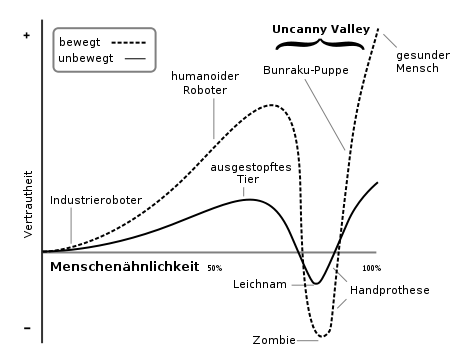
\includegraphics[width=1.0\textwidth]{bilder/3_uncannyValley.png}
    \caption{Das Phänomen des unheimlichen Tals -  „uncanny valley“}
    \label{fig:uncanny-valley}
\end{figure}

Es wird verwendet um zu zeigen, dass die Akzeptanz gegenüber technisch simuliertem Verhalten vom Realitätsgehalt abhängt. Dabei verzeichnet eine Annäherung an das menschenähnliche Verhalten innerhalb eines bestimmten Bereiches einen signifikanten Einbruch dieser Akzeptanz.

\section{Requirements Engineering}
\label{sec:requirements-engineering}
In diesem Kapitel wird die Anforderungsanalyse unter Berücksichtigung der genannten Aspekte beschrieben. Dieser Schritt ist äußerst wichtig, um das System auf die im Fokus liegende Zielgruppe abzustimmen. Die Methoden, der Grund ihrer Anwendung und die Ergebnisse sind in den jeweiligen Unterkapiteln näher erklärt.

\subsection{Umfrage}
\label{subsec:online-umfrage}
Um sich einen groben Überblick zu verschaffen soll zunächst geklärt werden warum und in welchem Umfang Online-Banking verwendet wird. Um das Ergebnis aufgrund einer möglichen Voreingenommenheit gegenüber \acp{VUI} nicht zu verfälschen, soll dafür der Zusammenhang mit diesen unerwähnt bleiben. Wie bereits festgestellt, besteht die Zielgruppe aus Personen, die ihre Bankgeschäfte über Online-Banking abwickeln. Dennoch wäre es sehr interessant festzustellen was die Gründe für diejenigen sind, die Online-Banking nicht nutzen.\\
Um ein breiteres Spektrum an Information zu erhalten, werden hierfür quantitative Daten über eine anonyme Online Umfrage gesammelt. Diese sollen auch helfen die Intention der Benutzer bei der Ausführung bestimmter Funktionen zu ergründen. Für die Durchführung der Umfrage stehen die folgenden drei Anwendungen in der engeren Auswahl. 

\begin{itemize}
    \item Google Forms \cite{google-forms}
    \item Survey Monkey \cite{survey-monkey}
    \item Umfrage Online \cite{umfrage-online}
\end{itemize}

Tabelle \ref{tab:umfrage-toolauswahl} stellt den Funktionsumfang der Anwendungen mit den Anforderungen an diesen gegenüber.

\begin{table}[!htb]
\centering
 \begin{tabular}{ | m{5cm} || C{2cm}| C{2cm} | C{2cm} |} 
 \hline
 Anforderungen & Google Forms & Survey Monkey & Umfrage Online
 \\
 \hhline{=::===}
 16 Fragen & \cmark & \danger & \cmark\\ 
 \hline Umfragelogik & \xmark & \danger & \cmark\\
 \hline Auswertung & \cmark & \cmark & \cmark\\
 \hline Anonymisierung & \cmark & \cmark & \cmark\\ 
 \hline Mehrfache Teilnahme unterbinden & \danger & \cmark & \cmark\\ 
 \hline
\end{tabular}
\caption{Auswahlhilfe für die Anwendung zur Durchführung der Umfrage}
\label{tab:umfrage-toolauswahl}
\end{table}

Die Anforderungen resultieren \ua aus dem erstellten Fragebogen, welcher zusammen mit den Antworten aus Gründen der besseren Lesbarkeit und des Leseflusses im \nameref{sec:Anhang} unter Kapitel \ref{sec:ausfuehrung-online-umfrage} zu finden ist. Erfüllte Anforderungen sind in Tabelle \ref{tab:umfrage-toolauswahl} mit grünen Haken, nicht erfüllte mit einem roten „X“, versehen. Die Warndreiecke sagen aus, dass diese Anforderungen nur unter bestimmten Bedingungen erfüllt werden. Im Fall von Survey Monkey können diese nur mit zusätzlichem Kostenaufwand erfüllt werden. Google Forms wiederum verlangt für das Unterbinden mehrfacher Teilnahmen pro Befragten, dass sich diese registrieren.\\
Wegen den aus Tabelle \ref{tab:umfrage-toolauswahl} ersichtlichen Gründen, fällt die Wahl auf die Anwendung Umfrage Online. Es erfüllt alle Voraussetzungen und kann außerdem ohne zusätzliche Kosten genutzt werden. Im Anschluss werden die wichtigsten Ergebnisse und Erkenntnisse zusammengefasst.\\
Der Prozentsatz der Online-Banking-Nutzer in der Umfrage unterscheidet sich deutlich von den in Kapitel \ref{sec:bankkonten-management} referenzierten Statistiken. Über 90 Prozent der Umfrage-Teilnehmer nutzen Online-Banking. Dies ist möglicherweise auf das Durchschnittsalter zurückzuführen. Wie aus Frage 16 ersichtlich ist, sind über 46 Prozent der Teilnehmer zwischen 18 und 30 Jahre alt. Nur knapp 12 Prozent sind älter als 50. Die Diskrepanz lässt sich also dadurch erklären, dass Personen im hohen Alter weniger geneigt sind ihre Bankgeschäfte online zu erledigen. Weiterhin kann die Umfrage nur von Personen mit einem Computer oder mobilen Endgerät durchgeführt werden. Dies kann ein weiterer Grund dafür sein.\\
Als Hauptgründe für die Nutzung von Online-Banking sind vor allem der schnelle Zugriff und die Bequemlichkeit bei der Verwendung genannt. An diesen zwei Kriterien kann man mit einem \ac{CUI} sehr gut ansetzen. Genau das sind mitunter große Vorteile dieser Systeme und Gründe für deren Einsatz.\\
Weiterhin werden die Intentionen der Nutzer beim Prüfen ihres Kontostandes \bzw ihrer Umsätze erfragt. Die am häufigsten genannten Intentionen sind Kontrolle und Überwachung des Guthabens. Dennoch gibt es sehr interessante Antworten, die man als Grundlage für weitere Anwendungsfälle nutzen kann. Darunter zu finden sind sinngemäß:

\begin{itemize}
    \item\textit{„Was kann ich mir noch leisten?“}
    \item\textit{„Gibt es Auffälligkeiten?“}
    \item\textit{„Ist mein Lohn/Gehalt schon da?“}
    \item\textit{„Habe ich Geld aus Gutschriften erhalten?“}
    \item\textit{„Ich möchte eine einfache Übersicht“}
\end{itemize}

Da viele Online-Banking-Plattformen auch den Handel mit Aktien \bzw das Verwalten eines Wertpapier Depots ermöglichen, sind auch diesbezüglich Fragen in die Umfrage eingeflossen. Anwendungsfälle aus dem Aktienbereich sind denkbare und sinnvolle Erweiterungsmöglichkeiten für ein Banking-\ac{CUI}. Da der Fokus der Arbeit auf dem Management von Bankkonten liegt werden diese Fälle nicht weiter ausgebaut, sondern nur als eine Möglichkeit zur Erweiterung gesehen.\\
Die Sicherheitsbedenken bei der Nutzung von Online-Banking sind sehr hoch. Knapp 80 Prozent der Befragten haben solche Bedenken. Gerade das ist auch bei der Entwicklung des \ac{CUI} ein sehr wichtiger Punkt, der im weiteren Verlauf der Arbeit aufgegriffen wird.\\
Des Weiteren wird nach Vorschlägen gefragt, wie die Verwendung der Online-Banking-Anwendungen effizienter laufen könnte. Unter den Antworten befinden sich sinngemäß auch Folgende:

\begin{itemize}
    \item\textit{„Mehrere Unterkonten in einem Konto, um Geld auf verschiedene Themen aufzuteilen“}
    \item\textit{„Bei Smartphone App Fingerabdruck statt Passwort bei Login“}
    \item\textit{„Sicherheit und Handling verbessern“}
    \item\textit{„Zugriff auf alle Sparbücher und Konten“}
    \item\textit{„Überweisungen über Handy App mit digitalem Überweisungsformular, dass man nur noch bestätigen muss“}
\end{itemize}

Unterkonten können mit den in Kapitel \ref{sec:bankkonten-management} erwähnten Sparzielen verglichen werden. Ebenso stimmt der Punkt Zugriff auf alle Sparbücher und Konten mit dem Begriff des Multibankings aus dem gleichen Kapitel überein.\\
Die hier erlangten Intentionen und Erkenntnisse werden im weiteren Verlauf der Arbeit aufgegriffen, genauer betrachtet und entwickelt.

\subsection{Interviews}
\label{subsec:interviews}
Durch die Erhebung der quantitativen Daten in Kapitel \ref{subsec:online-umfrage} wird ein allgemeiner Einblick in das Nutzungsverhalten beim Online-Banking gewährt. Für einen tieferen Einblick  sollen nun qualitative Daten gesammelt werden. Es soll auch konkret auf \acp{VUI} eingegangen werden. Dabei sind die Meinung und Akzeptanz von potentiellen Nutzern gegenüber dieser Systeme in Erfahrung zu bringen. Des Weiteren wäre es interessant zu sehen, wie Befragte auf die Kombination von Online-Banking und Sprachassistenzsystemen reagieren. Hier bietet die Methode des Interviews klare Vorteile. Es ist möglich auf die Antworten des Gegenübers einzugehen und im Fall von Unklarheiten nachzufragen. Wird das Interview von Angesicht zu Angesicht durchgeführt, können zusätzlich die Mimik und Gestik des Befragten Erkenntnisse liefern.\\
Aus den Kapiteln \ref{sec:conversational-user-interface} und \ref{sec:alexa-voice-service} ist bekannt, dass man einem \ac{CUI} Formulierungen vorgeben muss, damit es diese versteht. Ein Interview bietet auch eine gute Möglichkeit, nach solchen Formulierungen zu fragen.\\
Das Interview wird über einen Audiorekorder aufgezeichnet. Damit ist sichergestellt, dass Informationen nicht verloren gehen und eine Auswertung in schriftlicher Form nachträglich erfolgen kann. Dadurch ist der Interviewer in der Lage, parallel Notizen anzufertigen. Um die Anonymität der Befragten zu gewährleisten wird lediglich die schriftliche Ausarbeitung dokumentiert. Eine entsprechende Einverständniserklärung wird jedem Teilnehmer vor Durchführung des Interviews vorgelegt. Die Erklärung ist im \nameref{sec:Anhang} unter Kapitel \ref{sec:ausfuehrung-interview-einverstaendnis} zu finden, der Fragebogen selbst unter Kapitel \ref{sec:ausfuehrung-interview-fragebogen}. Wichtig bei der Durchführung eines Interviews sind die folgenden Verhaltensregeln: 

\begin{itemize}
    \item Einen neutralen und vertrauenswürdigen Eindruck vermitteln
    \item Jeden Befragten respektvoll behandeln
    \item Es gibt keine falschen Antworten
    \item Den Befragten nicht widersprechen
    \item Bei Unklarheiten nachfragen
\end{itemize}

Deren Einhaltung stellt sicher, dass die Gedanken und Meinungen des Nutzers erfasst und verstanden werden können. Es ist nicht zielführend dem Gegenüber die eigene Meinung näher zu bringen. Eine solche Beeinflussung verfälscht lediglich die Ergebnisse.\\ 
Vier Personen haben an den Interviews teilgenommen. Die schriftliche Auswertung ist im \nameref{sec:Anhang} unter Kapitel \ref{sec:ausfuehrung-interview-auswertung} dokumentiert. Diese liegt in einer sinngemäßen, stichpunktartigen Zusammenfassung vor. Die Reihenfolge der jeweiligen Antworten ist willkürlich gewählt und entspricht nicht der chronologischen Anordnung der Interviews. Für einen besseren Überblick werden die wichtigsten Ergebnisse hier zusammengefasst. Im Anschluss wird die Durchführung an sich rekapituliert.\\
Die Altersgruppe der Befragten liegt zwischen 22 und 26. Im Allgemeinen ist die Meinung der Befragten gegenüber \acp{VUI} eher skeptisch, befremdlich und mit großen Bedenken verbunden. Dennoch wird die Technologie durchaus als praktisch, zeitsparend und interessant erkannt. Die Erfahrung der Teilnehmer mit Sprachassistenten ist eher gering. Die Verteilung der Online-Banking-Nutzung spiegelt in etwa den Trend der Online Umfrage wider. Die Intentionen bei der Nutzung und auch die Sicherheitsbedenken unterscheiden sich nicht zu den Erkenntnissen aus der Umfrage. Gerade weil es um die Verbindung einer neuen Technologie mit einem ohnehin sicherheitskritischen Bereich wie Finanzen geht, ist die Skepsis groß. Die Teilnehmer geben an ihre Bankgeschäfte überwiegend alleine und in einem diskreten Umfeld durchzuführen. Durch das Erfragen von spezifischen Formulierungen zu Anwendungsfällen, können nur vereinzelte Ergebnisse erzielt werden. Die Bereitschaft zur Nutzung eines solchen Systems ist eher gering und mit Kriterien, wie \zB guten Bewertungen anderer Benutzer, verbunden.\\ 
Zusätzlich sind die folgenden Anmerkungen der Teilnehmer dazu gekommen:

\begin{itemize}
    \item Die Bereitstellung von Informationen bezüglich Datenschutz und verwendeter Sicherheitsstandards des Systems sind wünschenswert. Dies trägt maßgeblich zur Entscheidung für oder gegen die Nutzung bei
    
    \item Wegen des schnellen Zugriffs, ist eine Funktion für eine ebenso schnelle Kontoübersicht nützlich
    
    \item Bei Überweisungen soll das Verstandene noch einmal ausgegeben und vom Nutzer bestätigt werden, bevor die Überweisung durchgeführt wird
    
    \item Wird das Konto mit der getätigten Überweisung überzogen, soll das System den Nutzer vorher warnen
    
    \item Der Benutzer soll im Falle einer Buchung benachrichtigt werden
    
    \item Die Verwaltung von Finanzen ist ein seriöses Thema. Das System sollte den Benutzer nicht duzen.
\end{itemize}

Auch wenn die Erkenntnisse aus den konkreten Interview Fragen wenig überraschend sind, können dennoch wichtige Gesichtspunkte in die Entwicklung des Systems einfließen. Vor allem die zusätzlichen Vorschläge und Ideen der Befragten erscheinen äußerst sinnvoll und finden im weiteren Verlauf der Arbeit Verwendung.\\
Trotzdem gibt es auch etwas zu beanstanden. Das Alter der Befragten entspricht bei weitem nicht der kompletten Zielgruppe. Fragen nach Sprachbefehlen für konkrete Anwendungsfälle haben den Fluss der Konversation negativ beeinträchtigt. Daraus entstandene Verzögerungen haben zu sichtlich unangenehmenen Situationen geführt. Aufgrund dessen wurden Fragen übersprungen. Die Folge sind die wenigen Ergebnisse aus diesem Teil der Interviews. 

\subsection{Personas}
\label{subsec:personas}
Die Methode der Personas ist ein Instrument, um die unterschiedlichen Bedürfnisse der Benutzer zu modellieren und daraus passende Lösungen abzuleiten. Sie stellen prototypische Benutzer dar und verkörpern ihre unterschiedlichen Ziele, Verhaltensweisen und Eigenschaften, die im Hinblick auf das zu entwickelnde Produkt relevant sind \cite{richter-ux-compact}. Die Basis für deren Modellierung bilden die gesammelten Daten aus den vorangegangenen Kapiteln \ref{subsec:online-umfrage} und \ref{subsec:interviews}.\\
Personas sollen einfach verinnerlicht werden. Dazu kann man ihnen durchaus Namen, Bild, Alter und Charakterzüge zuweisen \cite{richter-ux-compact}. Aus Gründen der Lesbarkeit wird im Folgenden nur eine der Personas abgebildet. Zu den anderen wird lediglich eine Zusammenfassung gegeben. Die Abbildungen aller Personas sind im \nameref{sec:Anhang} unter Kapitel \ref{sec:anhang-personas} zu finden.\\\\
Abbildung \ref{fig:alena-meier} zeigt die Persona Alena Meier. Sie ist eine organisierte Frau, die parallel viele Konten zu verwalten hat. Um ihr einen schnellen Überblick zu gewährleisten, ist es wichtig die benötigten Informationen des jeweiligen Kontos gebündelt abrufbar zu machen. Gleichzeitig muss sie die Zahlungen ihrer Mieter im Auge behalten. Um das zu schaffen ist sie auf Technik angewiesen. Da ihr mit der Arbeit und ihren Finanzgeschäften nicht viel Zeit übrig bleibt, vergeudet sie diese nur ungern an unausgereifte Technik.

\begin{figure}[!htb]
    \centering
    \fbox{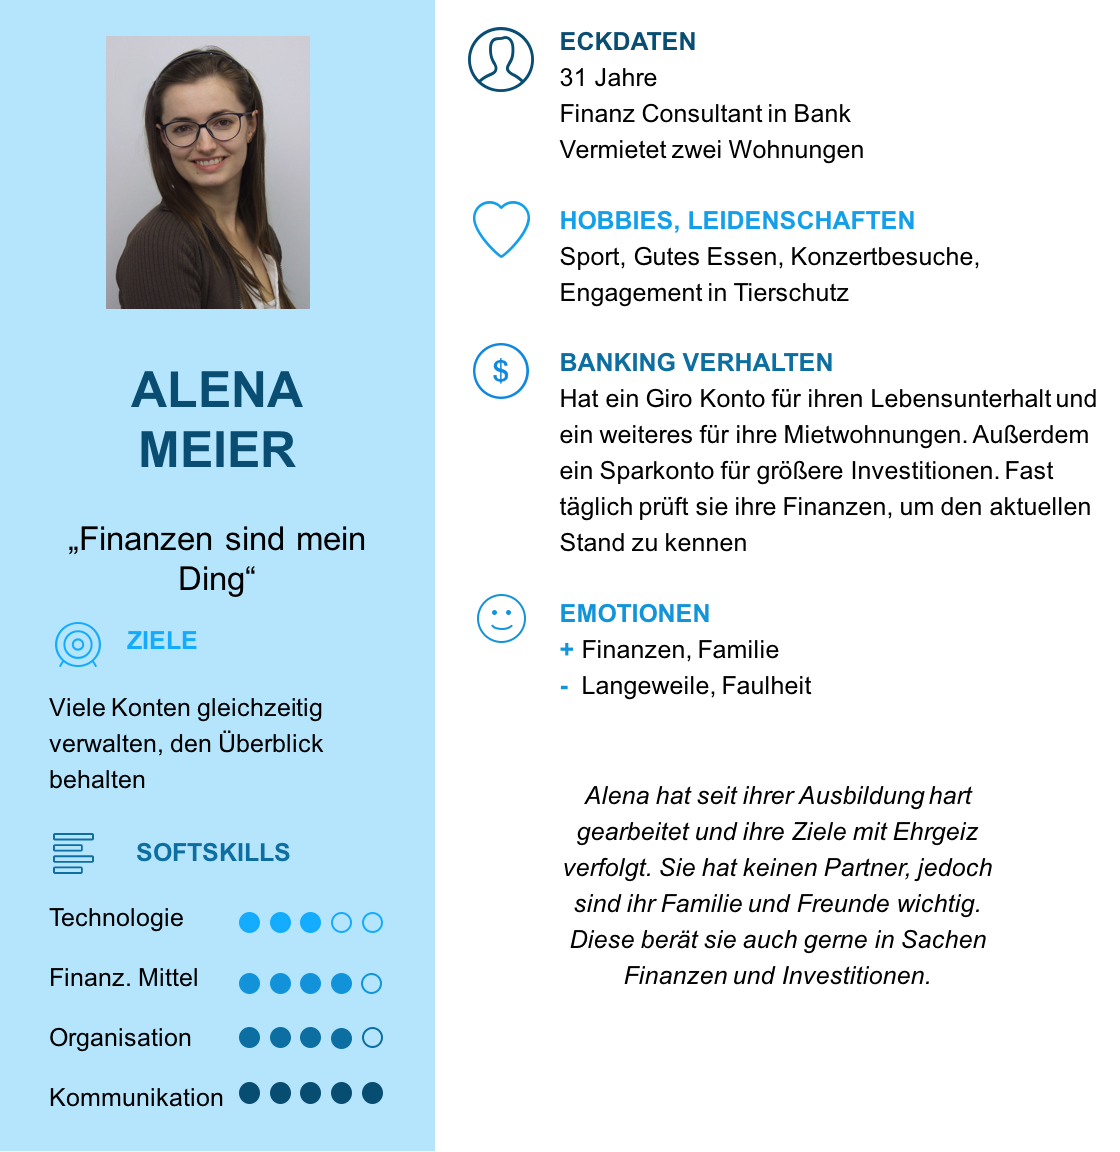
\includegraphics[width=1.0\textwidth]{bilder/3_alenaMeier.png}}
    \caption{Persona Alena Meier}
    \label{fig:alena-meier}
\end{figure}

Josef Lech aus Abbildung \ref{fig:robert-trier} kann durch seine körperliche Einschränkung nicht mehr den gewohnten Weg zur Bank nehmen. Er kommt nur schwer mit neuer Technik zurecht. Die Verwendung einer Online-Banking-Plattform ist ihm zu kompliziert. Ein \ac{VUI} kann hier einen guten Ansatz bilden. Über natürliche Sprache fällt es dem Rentner eventuell einfacher, seine Bankgeschäfte zu erledigen. Die Ausgaben des Banking Skills müssen aussagekräftig und hilfreich sein, damit dieser für Josef nutzbar wird.\\\\
Abbildung \ref{fig:robert-trier} zeigt die Persona Robert Trier, der großes Interesse daran hat neue Technologien zu verwenden. Als Fachmann weiß er aber auch, dass Datenschutz und Sicherheit äußerst wichtig sind. Bevor er neue Technik nutzt, erkundigt er sich über verwendete Sicherheitsstandards. Unbefugten darf es nicht möglich sein sensible Daten zu entwenden.\\\\
Die Persona Daniela Friedmann aus Abbildung \ref{fig:daniela-friedmann} muss ihr Konto ständig im Blick haben, damit sie es beim Ausgehen mit Freunden nicht überzieht. Dennoch möchte sie nicht jeden Tag daran erinnert werden, dass sie wenig Geld hat. Wegen der hin und wieder vorkommenden Indiskretion ihrer WG Mitbewohner, sind auditive Ausgaben von sensiblen Daten eher schwierig. Es muss eine Möglichkeit geben das zu umgehen. Außerdem muss im Falle ihrer Abwesenheit gewährleistet sein, dass kein anderer Zugriff auf ihre Daten erhält.\\\\
Das Modellieren der Personas liefert wichtige Erkenntnisse. Nicht nur Bedürfnisse und Ziele der einzelnen Personas können das Konzept bereichern. Auch der Nutzungskontext kann besser verstanden werden. Situationen, in denen das Produkt verwendet wird werden sichtbar. Darunter auch solche, die die Nutzung einschränken oder auch unmöglich machen. Das folgende Kapitel \ref{subsec:user-stories} beschreibt die Entwicklung der \textit{User Stories}, die aus den empirischen Daten und dem aktuellen Verständnis für die Zielgruppe resultieren.

\subsection{User Stories}
\label{subsec:user-stories}
Vor dem Einsatz eines \ac{CUI} ist immer zu evaluieren, welchen Mehrwert man mit dessen Einsatz für potentielle Benutzer generiert. Daher stellt sich in diesem Fall nicht die Frage, ob ein \ac{CUI} eine grafische Online-Banking-Anwendung ablösen kann. Es ist vielmehr als eine Ergänzung zu sehen. Eine, die für bestimmte Anwendungsfälle Vorteile bietet. Es gilt genau zu überlegen welche Funktionen hier sinnvoll sind und welche nicht.\\
Dieses Kapitel beschreibt den Funktionsumfang des Banking-Skills in Form von \textit{User Stories}. Sie basieren auf den Ergebnissen der vergangenen Kapitel \ref{subsec:online-umfrage} bis \ref{subsec:personas}. Wie ein \textit{Use Case} beschreibt auch die \textit{User Story} eine Funktion aus Sicht des Nutzers. Der Unterschied liegt in der Granularität. Use Cases beschreiben den Vorgang feingranularer. Aus User Stories wird jedoch die Intention der Benutzer direkt erkenntlich, was hier auch der Grund für deren Verwendung ist.\\
Aus Übersichtszwecken und da sich die User Stories im weiteren Verlauf der Arbeit ändern können, ist eine komplette Liste im \nameref{sec:Anhang} unter Kapitel \ref{sec:anhang-user-stories} zu finden. Hier wird lediglich ein Überblick über die Kernfunktionen des Systems gegeben.

\begin{itemize}
    \item\textbf{Hilfe Funktion}: Die Hilfe kann einem Benutzer vermitteln, welche Funktionen verwendet werden können und über welche Formulierungen er diese aufrufen kann. Denkbar ist hier auch eine kontextbezogene Hilfe. Das soll vor allem den Benutzern helfen, die \acp{VUI} \bzw den Skill zum ersten Mal verwenden. Auch Nutzer, die ihn nur selten verwenden können davon profitieren.
    
    \item\textbf{Profile verwalten/Authentifizierung}: Da jeder Benutzer mit den eigenen Bankkonten und Daten arbeitet, ist ein Authentifizierungsmechanismus unabdingbar. Nutzern muss es möglich sein sich zu registrieren und das angelegte Profil zu verwalten.
    
    \item\textbf{Bankkonten verknüpfen}: Damit Nutzer ihre Bankkonten verwalten können, müssen diese zunächst an das System angebunden werden.
    
    \item\textbf{Hauptkonto wählen}: Aus den in Kapitel \ref{sec:bankkonten-management} genannten Gründen müssen Nutzer in der Lage sein, eines der verknüpften Konten als Hauptkonto zu setzen. 
    
    \item\textbf{Vorlagen verwalten}: Damit Überweisungen schnell und einfach über Spracheingaben durchgeführt werden können soll es möglich sein, Zielkonten als Vorlagen zu speichern. Nutzern ist es möglich diesen Vorlagen Namen zuzuweisen, um diese zu adressieren. 
    
    \item\textbf{Kontostand}: Benutzern soll es möglich sein, den aktuellen Kontostand abzurufen.
    
    \item\textbf{Transaktion}: Unter Verwendung einer Vorlage und eines Geldbetrages können Benutzer Überweisungen durchführen, wie zum Beispiel „Überweise \textit{50} Euro an \textit{Julian}“. Das Verstandene muss vom System wiederholt und vom Benutzer bestätigt werden, bevor die Überweisung durchgeführt wird. Des Weiteren muss eine Möglichkeit zur \textit{\ac{TAN}} Eingabe geschaffen werden, um die Transaktion zu authentifizieren. Das Ausfüllen von Überweisungsträgern unter Angabe des \textit{\ac{IBAN}} soll nicht möglich sein. Die Eingabe langer Buchstaben und Ziffer Kombinationen über Sprache kann vor allem bei Eingabefehlern schnell frustrieren. Dafür können Benutzer auf eine Online-Banking-Plattform \bzw Überweisungsträger aus Papier zurückgreifen. Das ist ein gutes Beispiel für die Koexistenz eines \ac{CUI} mit bestehenden \acp{GUI}.
    
    \item\textbf{Gehaltseingang prüfen}: Als eine der Intentionen aus der \nameref{subsec:online-umfrage}, sollen Nutzer prüfen können, ob ihr Gehalt für die aktuelle Finanzperiode bereits eingegangen ist. Ein Vorteil dieser Ausgabe ist, dass es sich dabei nicht um sensible Daten handelt. Die Beantwortung soll lediglich eine Art „ja“ oder „nein“ beinhalten. Die Höhe des Gehaltes wird dabei nicht genannt. 
    
    \item\textbf{Budget abrufen}: Teilnehmer der \nameref{subsec:online-umfrage} aus Kapitel \ref{subsec:online-umfrage} und der \nameref{subsec:interviews} aus Kapitel \ref{subsec:interviews} geben an, dass ein schneller Überblick über das Konto wünschenswert ist. Das Budget verrät, wie viel am Ende der aktuellen Finanzperiode auf dem Konto bleibt. Dies wird anhand des bisherigen Ausgabeverhaltens ermittelt. Benutzer sind dadurch in der Lage, ihr Verhalten gegebenenfalls anzupassen.
    
    \item\textbf{Fixkosten}: Abfragen zu Fixkosten komplettieren die Funktion des schnellen Überblicks und erlauben den Benutzern zu prüfen, wie viel Geld sie regelmäßig ausgeben. Beispiele hierfür sind „Miete“, „Strom-“ und „Heizkosten“.
    
    \item\textbf{Umsatzdaten}: Natürlich macht es wenig Sinn sämtliche Umsätze mehrerer Tage auszugeben. Das ist ein typisches Beispiel für einen schlechten \ac{CUI} Anwendungsfall. Lange, komplexe Listen können von einer grafischen Oberfläche wesentlich verständlicher und eleganter dargestellt werden. Dennoch können Nutzer durch gezielte Fragen schnell an Informationen kommen. Denkbar sind Abfragen zu bestimmten Zahlungsempfängern \bzw -sendern, Beträgen oder Verwendungszwecken. 
    
    \item\textbf{Sparziele verwalten}: Benutzern soll es möglich sein Sparziele zu verwalten. Damit können für bestimmte Themen Geld gespart werden.
\end{itemize}

Die hier beschriebenen Funktionalitäten spiegeln die Erkenntnisse aus den vorangegangenen Kapiteln wider. Dennoch ist sicherzustellen, dass die Daten auch richtig interpretiert werden. Zu diesem Zweck werden im Folgenden Nutzungsszenarien erstellt. Auf Basis dieser Szenarien werden in Kapitel \ref{sec:prototyping} User Tests durchgeführt, um die bisherigen Ergebnisse zu evaluieren.

\subsection{Szenarien}
\label{subsec:szenarien}
Anwendungsszenarien sind ein zentrales Element in der nutzerorientierten Entwicklung. Sie schlagen die Brücke zwischen den Anforderungen und dem Entwurf eines neuen Konzeptes. Szenarien beschreiben anhand realistischer Beispiele wie Benutzer mit dem zu entwickelnden Produkt interagieren \cite{richter-ux-compact}. Die in Kapitel \ref{subsec:user-stories} erschlossenen Funktionen sollen nun in solche Szenarien einfließen. Diese bilden dann die Grundlage der Benutzertests in Kapitel \ref{sec:prototyping}. Für die Entwicklung der Szenarien werden auch die modellierten Personas aus Kapitel \ref{subsec:personas} berücksichtigt.\\
Damit die Aufgaben so natürlich wie möglich wirken, müssen sie in sich plausibel sein. Unrealistische Vorgaben und Daten können Tests negativ beeinflussen. Auch zu viel Realität kann störend wirken. Szenarien mit zu vielen Details passen womöglich nicht auf die Testperson. Sind Aufgaben beispielsweise auf einen verheirateten Vater von zwei Kindern zugeschnitten, obwohl die Testperson alleinstehend lebt, kann sich diese nicht mit dem Szenario identifizieren. Dabei können wichtige Erkenntnisse verloren gehen. Es ist also darauf zu achten plausible Szenarien zu erstellen, die lediglich die grundlegenden Lebensumstände vorgeben. Aus diesem Grund sollen die verwendeten Personas nicht in allen Facetten als Vorlage dienen. Hierfür werden drei grundlegende Szenarien erstellt, die sich im weiteren Verlauf der Arbeit auch ändern oder ausbauen lassen. Der Lebensumstand soll wie erwähnt allgemein gehalten werden. Aus den modellierten Personas aus Kapitel \ref{subsec:personas} können die folgenden Lebensumstände erkannt werden:

\begin{itemize}
    \item\textit{Student}
    \item\textit{In Lebenspartnerschaft}
    \item\textit{Verheiratet}
\end{itemize}

Für diese werden entsprechende Szenarien und die damit verbundenen Aufgaben für die Tests entwickelt. Im Folgenden wird nur eines der Szenarien abgebildet. Eine Übersicht aller ist im \nameref{sec:Anhang} unter Kapitel \ref{sec:anhang-szenarien} gegeben.

\textbf{Studenten Szenario}\\
Auf Grundlage der Persona \textit{Daniela Friedmann} aus Abbildung \ref{fig:daniela-friedmann} und unter Berücksichtigung der oben genannten Vorgaben wird ein Szenario für Studenten erstellt. Abbildung \ref{fig:szenario-student} stellt es mit den Aufgaben für die User Tests dar. Bei der Wahl der Aufgaben wird versucht möglichst realistisch auf die Lebensumstände eines Studenten einzugehen. 

\textbf{Lebenspartnerschaft Szenario}\\
Für dieses Szenario dient die Persona \textit{Alena Meier} aus Abbildung \ref{fig:alena-meier-anhang} als Grundlage. Auch wenn sich diese nicht in einer Beziehung befindet, werden andere Gesichtspunkte wie das Einkommen und ihre Freizeitaktivitäten berücksichtigt. Abbildung \ref{fig:szenario-partner} zeigt das Ergebnis. 

\begin{figure}[!htb]
    \centering
    \fbox{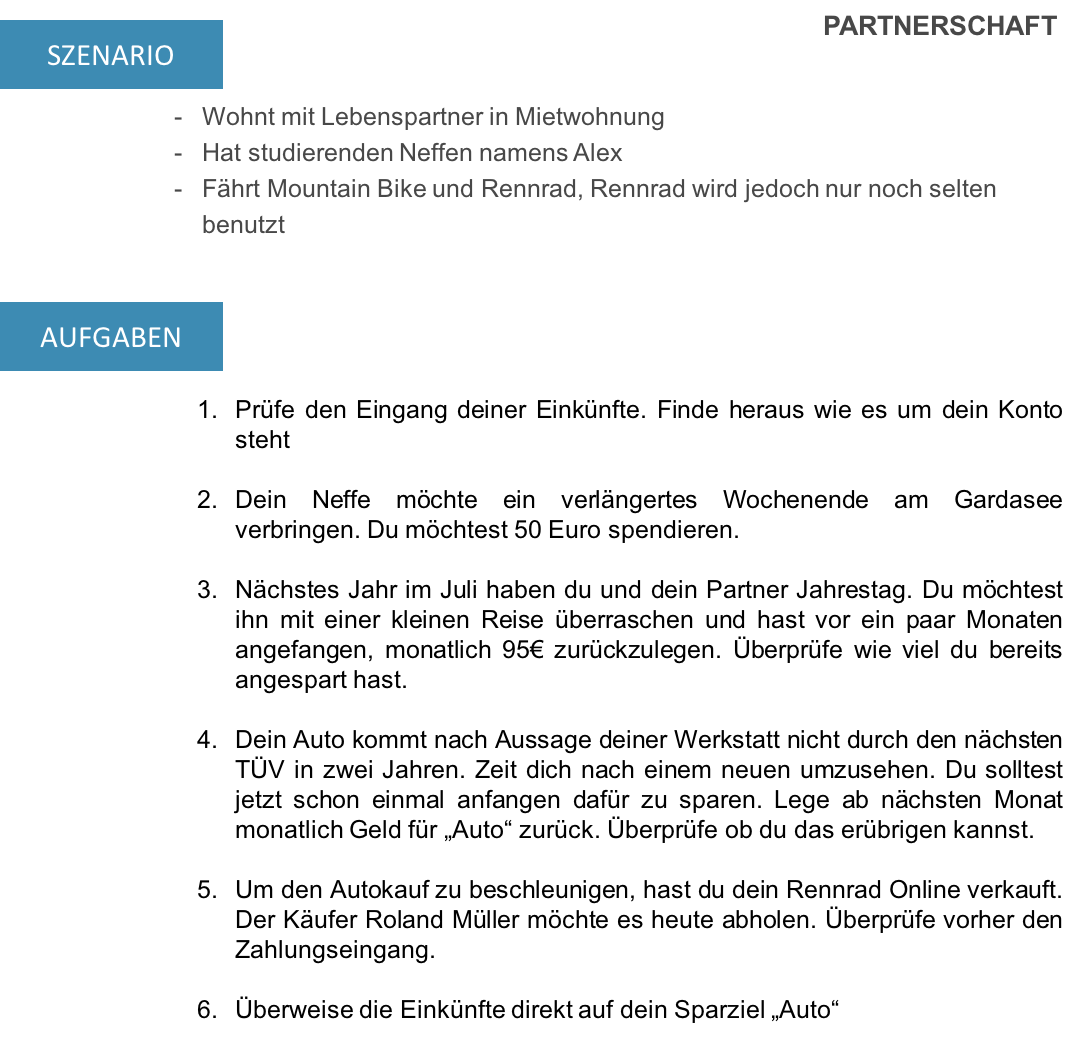
\includegraphics[width=1.0\textwidth]{bilder/3_szenarioPartner.png}}
    \caption{Partnerschaft Szenario}
    \label{fig:szenario-partner}
\end{figure}

\textbf{Verheiratet Szenario}\\
Als Vorlage dieses Szenarios wird die Persona \textit{Robert Trier} aus Abbildung \ref{fig:robert-trier} verwendet. Auch hier werden Lebensumstände, Einkommen und Hobbies für die Wahl der Aufgaben herangezogen. In Abbildung \ref{fig:szenario-verheiratet} sieht man Szenario und entsprechende Aufgaben.\\\\
Diese Szenarien sollen nun mit potentiellen Nutzern getestet werden. 

\section{Prototyping}
\label{sec:prototyping}
Im Usability Engineering wird Prototyping eingesetzt, um Produkte und Aspekte der Benutzerschnittstelle zu entwerfen, zu evaluieren und zu verbessern. Dies geschieht bevor ein lauffähiges System vorhanden ist. Beim Prototyping gibt es verschiedene Stufen. Diese beschreiben in wie weit der Prototyp dem zu entwickelnden Produkt in den folgenden Bereichen ähnelt:
\begin{itemize}
\item Funktionsumfang: Welche der vorgesehenen Funktionen der Prototyp zeigt
\item Funktionstiefe: Wie detailliert die Funktionen wiedergegeben werden
\item Darstellungstreue: Wie sehr das Erscheinungsbild dem Endprodukt ähnelt
\item Interaktivität: Wie interaktiv der Prototyp ist
\item Datengehalt: Ob dynamische oder statische Daten verwendet werden
\item Technische Reife: Wie viel der endgültigen Technologie des Endproduktes im Prototypen steckt.
\end{itemize}

Jeder Prototyp stellt einen Kompromiss zwischen notwendigem Aufwand und Zweck dar \cite{richter-ux-compact}. Anhand der aufgelisteten Bereiche, lassen sich Prototypen in die folgenden drei Stufen unterteilen:

\begin{itemize}
    \item\textit{\ac{LoFi}}: \ac{LoFi} ist vom eigentlichen Endprodukt am weitesten entfernt. Im Gegenzug ist der Kostenaufwand dieser Methode sehr gering, da meist einfachste Werkzeuge zum Einsatz kommen. Bei grafischen Oberflächen wird diese Form des Prototyping oft mit Papier und Stift angewandt. Dabei werden die einzelnen Oberflächen auf Papier skizziert. Mit diesen Papierprototypen lassen sich \zB erste Bedienkonzepte der Oberfläche testen. In einem Test navigiert die Testperson über die Papierskizzen, die von einem Helfer entsprechend der Bedienlogik ausgetauscht werden.
    
    \item\textit{\ac{MiFi}}: Interaktivität und Erscheinung eines \ac{MiFi} Prototypen sind näher am Endprodukt als \ac{LoFi}. Hier können bereits digitale, interaktive Designs von Oberflächen zum Einsatz kommen. Benötigte Daten und komplexe Funktionalität werden meist noch vorgetäuscht (engl. \textit{gemockt}).
    
    \item\textit{\ac{HiFi})}: Ein \ac{HiFi} Prototyp ist dem Endprodukt sehr ähnlich. Hier kann es sich tatsächlich um ein funktionierendes System handeln. Möglicherweise ist es im Funktionsumfang eingeschränkt oder benötigte Daten werden noch gemockt. Oft kommen dabei bereits die Technologien zum Einsatz, die Teil des zu entwickelnden Produktes sind.
\end{itemize}

Der im Zuge dieser Arbeit entwickelte Banking-Skill, kann also als ein \ac{HiFi} Prototyp bezeichnet werden. Wie bereits erwähnt, wird für die Umsetzung in Kapitel \ref{cha:umsetzung} zunächst ein Konzept ausgearbeitet. Da die Bearbeitungszeit bei der Durchführung der Arbeit ein Faktor ist, soll hierfür entweder \ac{LoFi} oder \ac{MiFi} Prototyping verwendet werden. Mit Hilfe der passenden Werkzeuge und Methoden wird das Konzept durch Tests mit potentiellen Nutzern schrittweise ausgebaut. Für die Wahl eines passenden Tools beschreibt Kapitel \ref{subsec:anforderungen-prototyping} die Anforderungen.

\subsection{Anforderungen an ein Prototyping Tool}
\label{subsec:anforderungen-prototyping}
Bevor eine passende Anwendung gewählt wird, müssen die Anforderung an diese definiert werden.
\begin{itemize}
\item Schnelle Änderungen:\\
Es ist wichtig zu erkennen was für die Nutzer funktioniert. Noch wichtiger ist früh zu erkennen was nicht funktioniert -- Stichwort \textit{fail early}. Das heißt die Anwendung soll die Möglichkeit bieten, Ideen schnell auszuprobieren und diese gegebenenfalls zu verwerfen \bzw weiterzuverfolgen. Als Folge dessen ist darauf zu achten, dass Änderungen im Konzept keine Änderungen von Quelltext nach sich ziehen.

\item Konversationsfluss entstehen lassen:\\
Die Ergebnisse der Tests sollen möglichst realitätsnah sein, um das Konzept sinnvoll zu erweitern. Um das zu erreichen, muss die Anwendung das Aufkommen eines Konversationsflusses ermöglichen. Die Anwendung ist dabei an die technischen Möglichkeiten von Alexa auszurichten. Dazu zählen die Verzögerungen zwischen der Frage einer Testperson und der entsprechenden Antwort vom System. Des Weiteren muss es möglich sein Gegenfragen zu stellen. Für die Durchführung der Aufgaben aus den Szenarien in Kapitel \ref{subsec:szenarien} ist dies essenziell. Werden beispielsweise die benötigten Informationen einer Überweisung nicht vom Nutzer eingegeben, muss das System entsprechend nachfragen.

\item Unterstützung der Sprache:\\
Der Banking Skill wird in Deutsch entwickelt. Daher ist das Verstehen von Formulierungen in deutscher Sprache notwendig. 
\end{itemize}

Im Anschluss wird eine entsprechende Anwendung gesucht. Die hier genannten Anforderungen zielen vor allem auf geringen Zeitaufwand in der Verwendung ab. Diese Tatsache lässt auf ein \ac{MiFi} Prototyping Tool schließen.

\subsection{Existierende Anwendungen}
\label{subsec:prototyping-existierende-anwendungen}
Anders als im Bereich der \ac{GUI} Entwicklung, ist die Auswahl der \ac{CUI}-\ac{MiFi}-Anwendungen überschaubar. Im Folgenden werden drei dieser Anwendungen näher betrachtet:

\begin{itemize}
    \item\textit{Sayspring}: Eine Web-Anwendung für das Entwerfen und Prototyping von \acp{VUI} ohne Programmieraufwand \cite{sayspring}.
    \item\textit{API.AI (heute Dialogflow)}: Eigentlich ein Framework für die Entwicklung von Chatbots und \acp{VUI}. Es kann auch als Prototyping Tool zweckentfremdet werden \cite{dialogflow-api-ai}. 
    \item\textit{Wit.ai}: Ähnlich wie API.AI, handelt es sich um ein Framework für die Entwicklung von Chatbots und \acp{VUI} \cite{wit-ai}.
\end{itemize}

Als Entscheidungshilfe stellt Tabelle \ref{tab:vergleich-mifi-toolauswahl} die Anforderungen aus Kapitel \ref{subsec:anforderungen-prototyping} den genannten Anwendungen gegenüber.

\begin{table}[!htb]
\centering
 \begin{tabular}{ | m{5cm} || C{2cm}| C{2cm} | C{2cm} |} 
 \hline
 Anforderungen & Sayspring & API.AI & Wit.ai
 \\
 \hhline{=::===}
 Schnelle Änderungen & \danger & \xmark & \xmark\\ \hline
 Konversationsfluss & \danger & \danger & \danger\\\hline 
 Sprachunterstützung & \xmark & \cmark & \cmark\\\hline 
\end{tabular}
\caption{Auswahlhilfe für Anwendungen aus dem \ac{CUI} Mid-Fidelity-Prototyping}
\label{tab:vergleich-mifi-toolauswahl}
\end{table}

Der Vergleich zeigt, dass keine der Anwendungen alle Anforderungen erfüllen kann.\\
Mit Sayspring kann man Konversationen schnell und einfach aufbauen, jedoch kann nur das verstanden werden was man modelliert. Ein echter Konversationsfluss kann somit nicht aufgebaut werden. Änderungen lassen sich zunächst schnell vornehmen. Bei zunehmender Komplexität wird die Bearbeitung eher mühsam. Der größte Nachteil von Sayspring ist allerdings die Sprache. Zum Zeitpunkt der Evaluierung unterstützt es lediglich englischsprachige Projekte. Deutsch wird erst seit dem 05.09.2017 unterstützt \cite{sayspring-german-support}. Abbildung \ref{fig:sayspring-gui} zeigt die Oberfläche der Web-Anwendung mit bereits erstellten Dialog Szenarien.

\begin{figure}[!htb]
    \centering
    \fbox{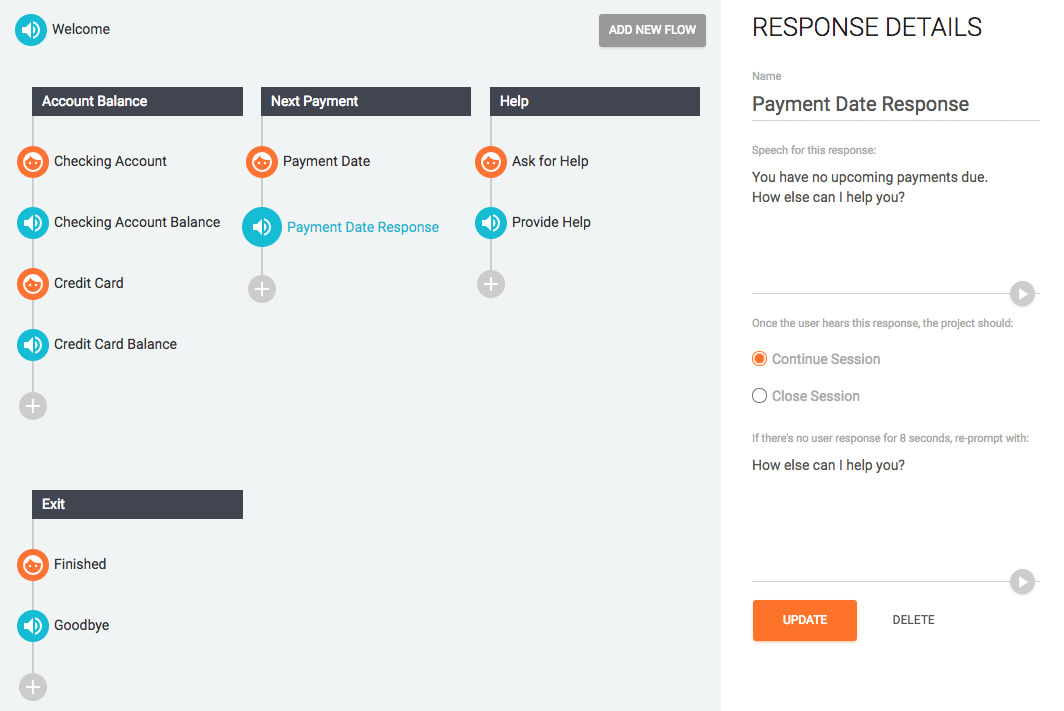
\includegraphics[width=0.8\textwidth]{bilder/3_sayspringGui.png}}
    \caption{Oberfläche der Sayspring Web-Anwendung}
    \label{fig:sayspring-gui}
\end{figure}

Anwendungen von API.AI bestehen, ähnlich wie Alexa, aus zwei Komponenten. Einer Interaction Model ähnlichen und einer Logikkomponente. Das Model muss ebenfalls mit Intents und Formulierungen konfiguriert werden. Auch wenn die Eingabe komfortabel ist sind Änderungen bei komplexen Projekten eher langsam umzusetzen. Hinzu kommt, dass die Logikkomponente implementiert werden muss. Logische Änderungen im Konzept sind also mit viel Aufwand verbunden. Auch hier kann die Konversation gut modelliert werden. Dennoch besteht hier das gleiche Problem wie bei Sayspring. Ein echter Fluss kann durch das eingeschränkte Verständnis nur schwer aufkommen.\\
Wit.ai ähnelt API.AI hinsichtlich Funktionsweise und Konfiguration über die Oberfläche. Auch hier muss Logik implementiert werden. Hervorzuheben ist, dass Wit.ai bereits zum Zeitpunkt der Evaluierung viele Sprachen unterstützt. Da keine der \ac{MiFi} Anwendungen passend erscheint, wird im folgenden Kapitel nach einer anderen Möglichkeit gesucht.

\subsection{Entstehung einer Prototyping Toolchain}
\label{subsec:prototyping-entstehung-toolchain}
Die Anwendungen aus Kapitel \ref{subsec:prototyping-existierende-anwendungen} können gemäß den Anforderungen aus Kapitel \ref{subsec:anforderungen-prototyping} nicht verwendet werden. Aus diesem Grund werden zunächst Methoden aus dem \ac{LoFi} Bereich näher betrachtet. Ähnlich wie bei der Entwicklung von \acp{GUI} kann man auch hier auf Stift und Papier zurückgreifen. Statt Oberflächen skizziert man Dialoge. Ähnlich wie ein Filmskript stellen sie Ausschnitte einer Interaktion dar \cite{pearl-design-vui}. Geschriebene Dialoge kann man mit einer einfachen Methode testen. Diese ist unter dem Namen \textit{\ac{WOz}} oder auch \textit{Wizard-of-Technique} bekannt. Bei \ac{WOz} Tests ist das eigentliche System noch nicht verfügbar. Stattdessen erweckt ein „Mensch hinter dem Vorhang“ den Eindruck eines funktionierenden Systems \cite{pearl-design-vui}. Für \ac{LoFi}-Prototyping kann ein \ac{WOz} Test gemäß Abbildung \ref{fig:woz-lofi} aufgebaut werden.

\begin{figure}[!htb]
    \centering
    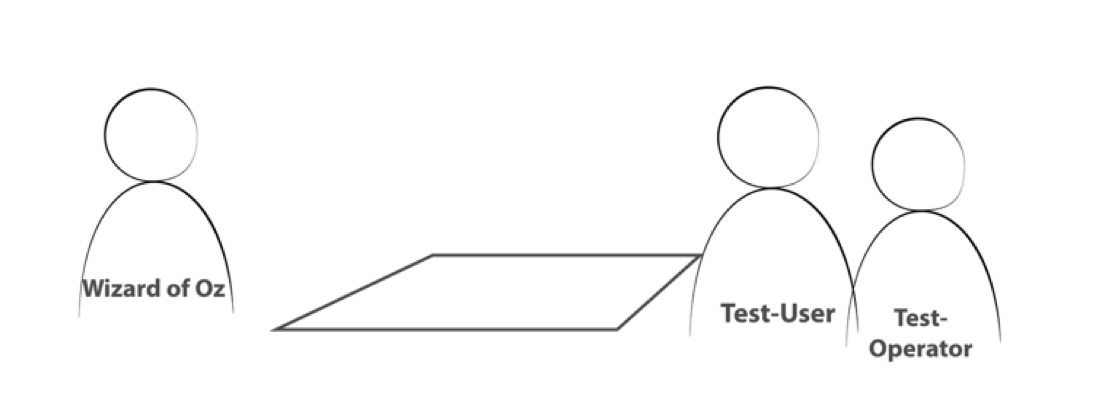
\includegraphics[width=1.0\textwidth]{bilder/3_wozLoFi.png}
    \caption{Low-Fidelity-Prototyping Test auf Basis von Wizard-of-Oz}
    \label{fig:woz-lofi}
\end{figure}

Der \ac{WOz} sitzt auf einer Seite eines Tisches, während die Testperson auf der anderen Seite sitzt. Der Test-Operator stellt der Testperson Aufgaben und betreut diese bei auftretenden Fragen. Die Testperson stellt dem \ac{WOz} für die Erfüllung der Aufgaben Fragen, die der \ac{WOz} entsprechend dem vorher festgelegten Skript beantwortet. Der Operator macht dabei Notizen zur Durchführung, dem Verlauf und den Ergebnissen des Tests.\\
Dieser Aufbau bringt Probleme mit sich. Der \ac{WOz} erhält über mehrere Kanäle Informationen, die dem Endprodukt nicht zur Verfügung stehen. Er kann die komplette Unterhaltung zwischen der Testperson und dem Operator mithören. Dadurch ist es möglich Schlüsse aus dem Kontext der Unterhaltung zu ziehen, die über das eigentliche Sprachkommando hinaus gehen. Weiterhin kann der \ac{WOz} den Fluss der Konversation durch Lachen oder Versprechen negativ beeinflussen. Er erhält weitere Informationen aus Mimik und Gestik der Testperson. Durch Aufstellen einer Trennwand kann man dem Problem entgegen wirken. Denkbar ist auch, den \ac{WOz} räumlich von den anderen Personen zu trennen. Abbildung \ref{fig:woz-lofi-voip} zeigt einen solchen Aufbau, in dem die Räume über Rechner mit \textit{\ac{VoIP}}-Anwendungen wie \zB Skype\footnote{https://www.skype.com/en, Abgerufen 31.10.2017} oder Google Hangout\footnote{https://hangouts.google.com, Abgerufen 31.10.2017} verbunden. 

\begin{figure}[!htb]
    \centering
    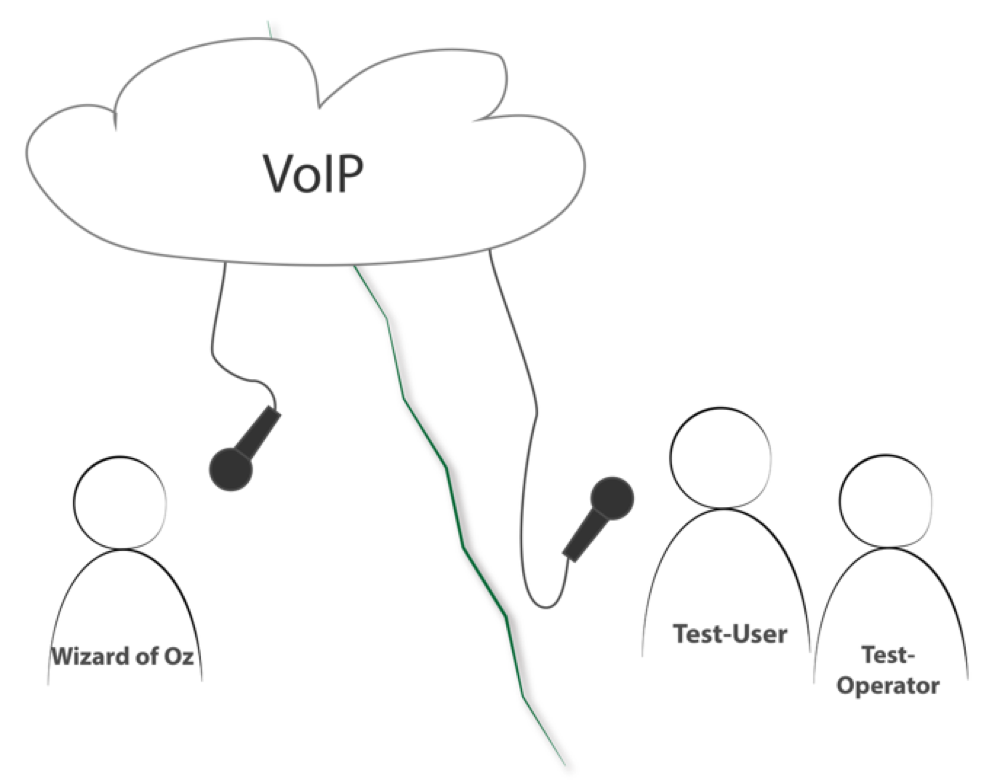
\includegraphics[width=0.8\textwidth]{bilder/3_wozLoFiVoIP.png}
    \caption{Wizard-of-Oz Low-Fidelity-Prototyping mit Voice over IP}
    \label{fig:woz-lofi-voip}
\end{figure}

Werden etwaige Kameras an den Rechnern deaktiviert, gibt es keine Informationen bezüglich Mimik und Gestik. Unter Einsatz eines Mikrofons mit Taster für die Sprachaktivierung sind auch die Unterhaltungen der Testperson und des Operators nicht zu hören. Diese Methode bringt viele Vorteile mit sich. Neben dem geringen Kosten- und Geräteaufwand, ist es zudem nicht nötig komplexe Technologien wie \ac{ASR} und \textit{NLP} zu verwenden oder gar zu implementieren. Da der \ac{WOz} ein Mensch ist, kann er alle Formulierungen der Testperson verstehen. Es besteht aber die Möglichkeit, dass sich der Wizard verspricht, lachen muss oder Sätze aus dem Skript nicht finden kann. Weitere Nachteile sind die zeitintensive Erstellung, Verwaltung und Erweiterung der Skripten. Bei zunehmender Komplexität wird es also schwieriger die Rolle des \ac{WOz} einzunehmen. Ein reibungsloser Ablauf ist wahrscheinlich mit intensiver Einarbeitung in das Skript verbunden. Werden die verbleibenden Probleme behoben, könnten mit diesem System sämtliche Anforderungen aus Kapitel \ref{subsec:anforderungen-prototyping} erfüllt werden. Abbildung \ref{fig:woz-weiterentwicklung} zeigt eine mögliche Weiterentwicklung dieser Gedanken.

\begin{figure}[!htb]
    \centering
    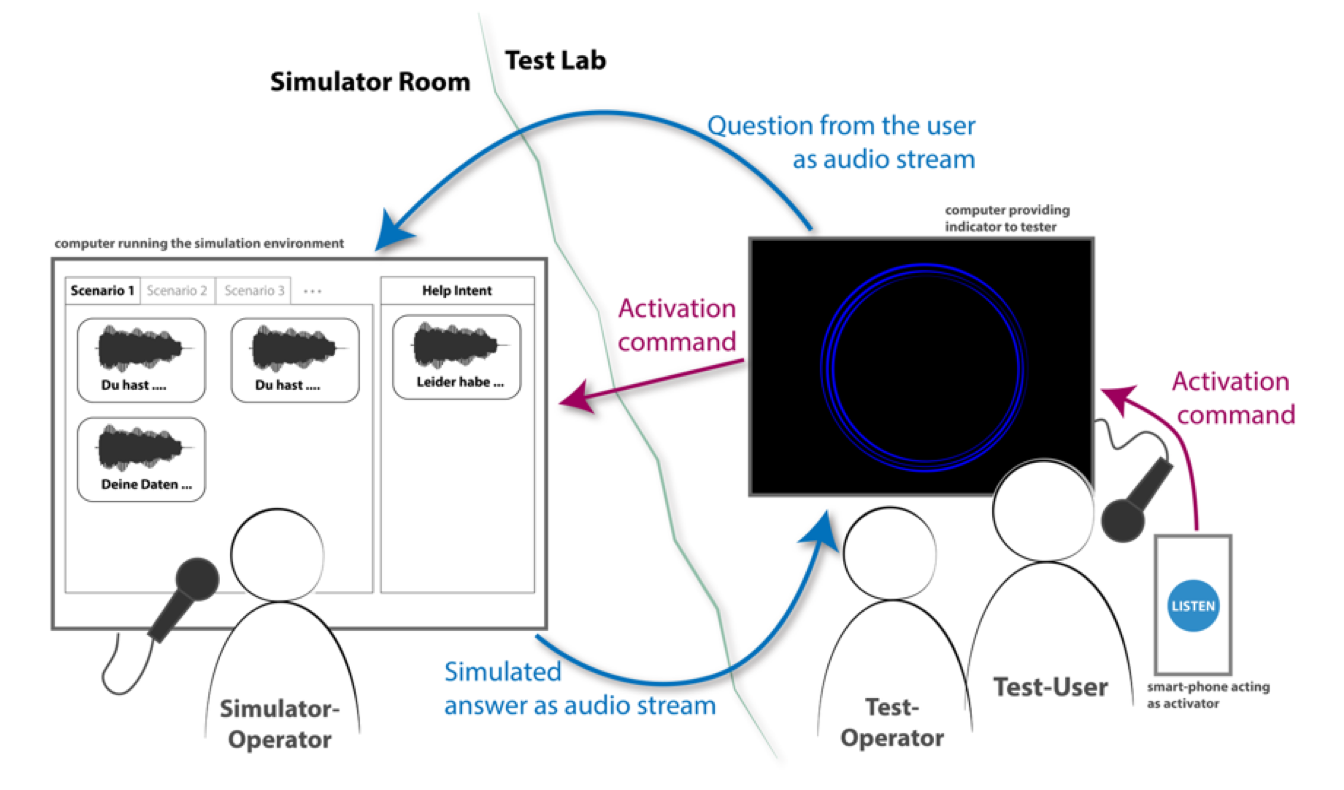
\includegraphics[width=1.0\textwidth]{bilder/3_wozFinal.png}
    \caption{Weiterentwicklung des Wizard-of-Oz Testaufbaus}
    \label{fig:woz-weiterentwicklung}
\end{figure}

Nach wie vor spricht die Testperson nach Aktivierung in ein Mikrofon und überträgt das Gesprochene an den \ac{WOz}. Dieser spricht die Antwortsätze nicht mehr selbst in ein Mikrofon. Er spielt zum richtigen Zeitpunkt vorher aufgenommene oder erzeugte Antwortsätze über eine Oberfläche ab. Diese werden als Audio an die Testperson im Labor übertragen. Bei entsprechender Gestaltung der Oberfläche findet sich der \ac{WOz} auch bei komplexen Tests zurecht. Gemäß Abbildung \ref{fig:woz-weiterentwicklung} lassen sich die Antworten in verschiedene Reiter unterteilen. Die gezeigte \ac{GUI} löst damit unter Umständen das Problem des Zurechtfindens und des Versprechens. Das Erstellen und vor allem schnelle Ändern des Dialog Skriptes sind nach wie vor kritisch. Zusätzlich zu der gezeigten Anwendung werden also noch weitere benötigt, die den Ablauf des Dialoges modellieren können und die Antwortsätze als Audio generieren. Das Ergebnis dieses Gedankens ist die in Abbildung \ref{fig:prototyping-toolchain} gezeigte Toolchain\footnote{Die Toolchain ist in Zusammenarbeit mit Steffen Blümm, dem fachlichen Betreuer der Arbeit entstanden}.

\begin{figure}[!htb]
    \centering
    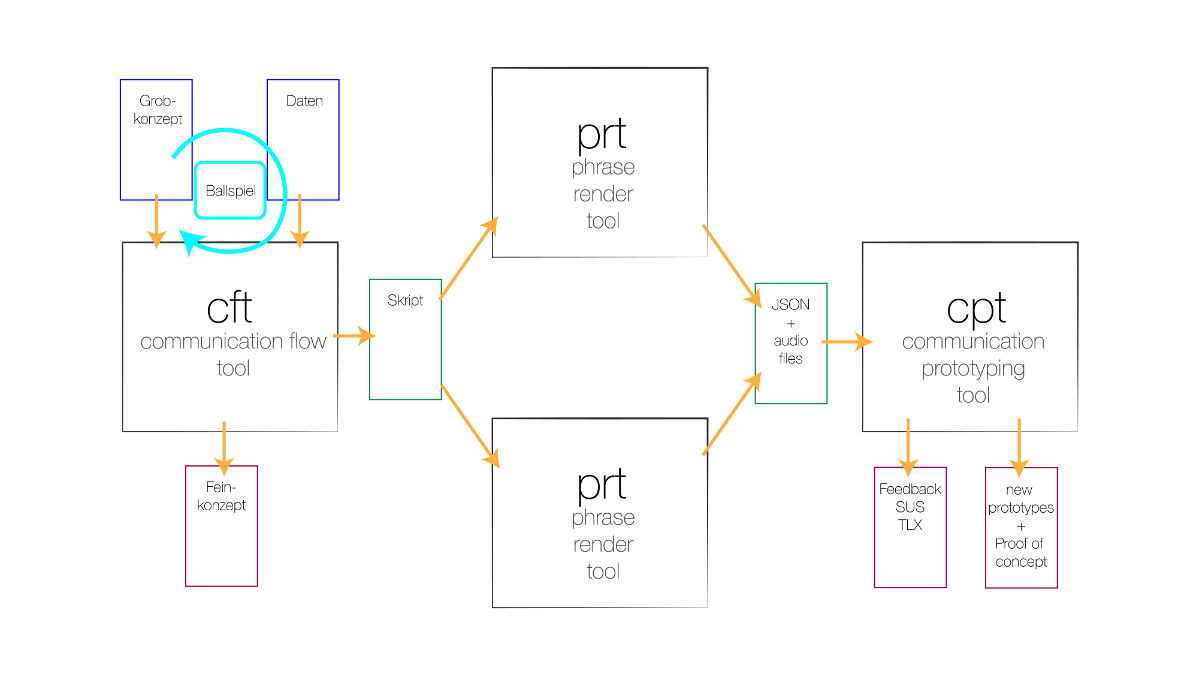
\includegraphics[width=1.0\textwidth]{bilder/3_toolchain-final.png}
    \caption{Prototyping Toolchain}
    \label{fig:prototyping-toolchain}
\end{figure}

Zunächst wird über ein Ballspiel ein Grobkonzept erarbeitet. Mit Hilfe eines Datensatzes (hier \zB Bank"~ \bzw Umsatzdaten) können sich zwei Personen gegenseitig einen „Ball“ zuwerfen. Das heißt abwechselnd die Rolle des Systems und des Benutzers einnehmen und dabei mögliche Fragen- und Antwortszenarien durchspielen. Das Ballspiel kann auch durch andere Methoden ersetzt werden, um ein Grobkonzept auszuarbeiten. Dieses Konzept wird händisch in das \textit{\ac{cft}} eingegeben. Hier können die Dialoge digital erstellt und bearbeitet werden. Denkbar für das \ac{cft} ist eine Sayspring ähnliche Oberfläche (\vgl Abbildung \ref{fig:sayspring-gui}). Im nächsten Schritt gibt das \ac{cft} den Dialogfluss in Form eines Datensatzes (\zB  in \textit{\ac{JSON}} Format) aus. Diese Ausgabedatei wird in das \textit{\ac{prt}} geladen. Es konvertiert gemäß der \ac{cft} Ausgabe die Antwortsätze über eine Art \ac{TTS} Synthese in Audio Dateien und reicht den \ac{cft} Datensatz weiter. Im letzten Schritt baut sich die \ac{WOz} Oberfläche mit Hilfe der \ac{prt} Ausgabe auf. Die generierten Audio Dateien und Szenarien werden geladen und der Test kann starten. Mit den Erkentnissen aus dem durchgeführten Test kann nun das Konzept über das \ac{cft} angepasst und ein weiterer Testlauf gestartet werden. Diese Vorgehensweise ist ein iterativer Prozess, der beliebig oft wiederholt werden kann. Aus dem Grobkonzept entsteht ein Feinkonzept, dass als Basis für die Implementierung genutzt wird.

\subsection{Umsetzung der Prototyping Toolchain}
\label{subsec:umsetzung-prototyping-toolchain}
Im Folgenden wird die Umsetzung der Prototyping Toolchain aus Abbildung \ref{fig:prototyping-toolchain} beschrieben. Da für die Durchführung der Tests vor allem das communication prototyping tool von Bedeutung ist, wird die Toolchain von rechts nach links entwickelt.\\

\textbf{communication prototyping tool}\\
Um den Zeitaufwand in Grenzen zu halten, ist das \ac{cpt} mit \textit{Max} von Cycling74 \cite{max-msp} umgesetzt, eine Art digitales Baukasten System. Max verbindet Objekte über virtuelle Leitungen, um interaktive Audio"~ und Grafiksysteme zu erstellen. Projekte in Max sind in sogenannten \textit{Patchern} organisiert. Sie beinhalten die verknüpften Objekte und sind ineinander verschachtelbar.\\
Das \ac{cpt} wird mit Max nach der Vorlage aus Abbildung \ref{fig:woz-weiterentwicklung} umgesetzt. Gemäß der Aufteilung in Simulator-Raum und Testlabor gibt es zwei Oberflächen \bzw Patcher, die auf den jeweiligen Rechnern laufen und Daten austauschen. Diese werden im Folgenden als \textit{Simulator-Panel} und \textit{Tester-Panel} bezeichnet. Abbildung \ref{fig:cpt-komponenten} zeigt eine Übersicht der Panele mit ihren Komponenten. 

\begin{figure}[!htb]
    \centering
    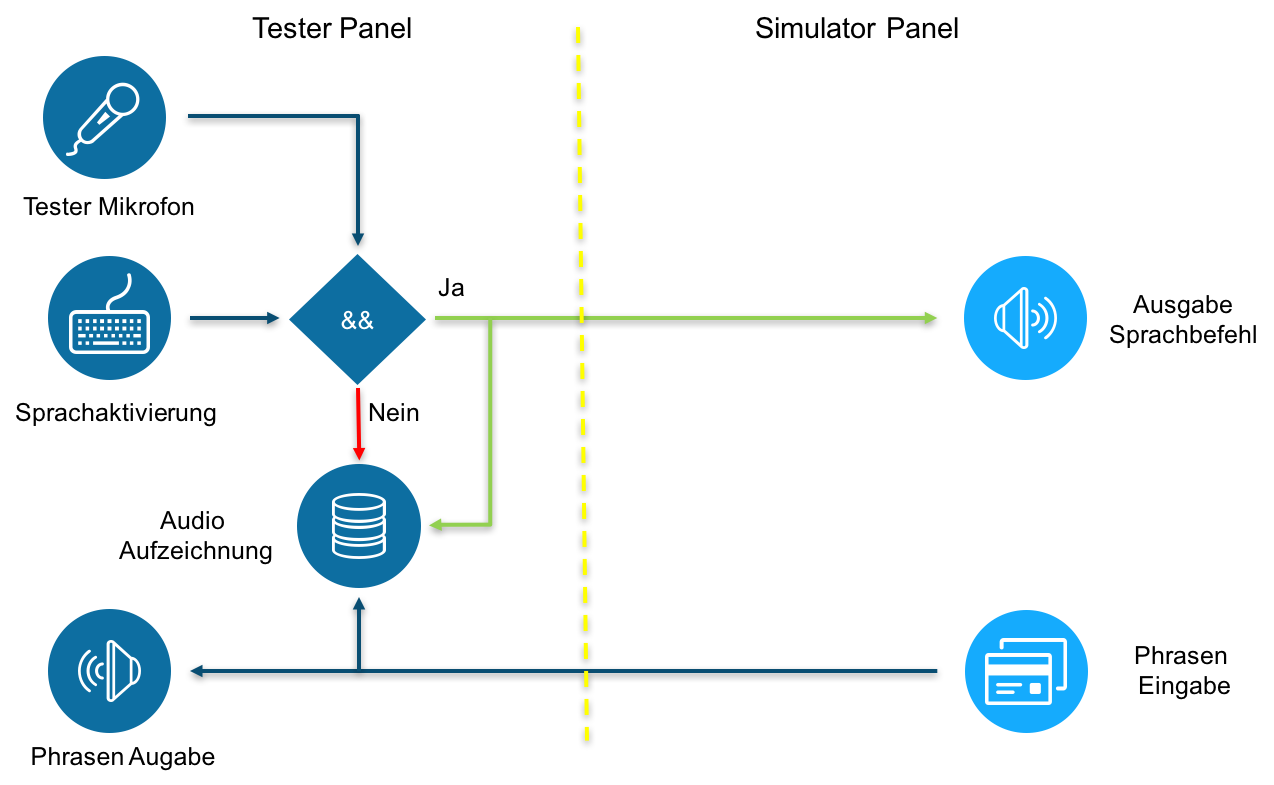
\includegraphics[width=1.0\textwidth]{bilder/3_cptKomponenten.png}
    \caption{Komponentenübersicht des Tester- und Simulator-Panels}
    \label{fig:cpt-komponenten}
\end{figure}

Das Tester-Panel ist für die Übertragung der Sprachbefehle des Testers und einer Möglichkeit der Sprachaktivierung zuständig. Zudem gibt es die Antwortphrasen aus, die vom Simulator-Panel übertragen werden. Diese Seite bildet die \ac{WOz} Oberfläche ab, die gemäß des Szenarios dynamisch aufgebaut wird. Sie gibt die Sprachbefehle des Testers aus und ermöglicht es diesem zu Antworten. Man greift dabei auf die generierten Audiodateien zurück. Um die Tests besser nachvollziehen zu können, werden zwei Audiospuren aufgenommen. Eine dieser Spuren zeichnet alles über das Tester Mikrofon (auch ohne Sprachaktivierung) und den Antwortphrasen auf. Die andere Spur zeichnet lediglich die Konversation zwischen Tester (mit Sprachacktivierung) und \ac{WOz} auf, um eine differenzierte Perspektive der Unterhaltung darzustellen. Im Folgenden ist die Umsetzung der Oberflächen in Max dokumentiert. Da der Fokus der Arbeit ein anderer ist, wird hier nur ein kurzer Überblick gegeben. Das komplette System mit den entsprechenden Quelltexten ist auf der CD unter \textit{„Quelltexte/cpt/“} zu finden. Abbildung \ref{fig:cpt-tester-panel} zeigt den Max Patcher für das Tester-Panel. 

\begin{figure}[!htb]
    \centering
    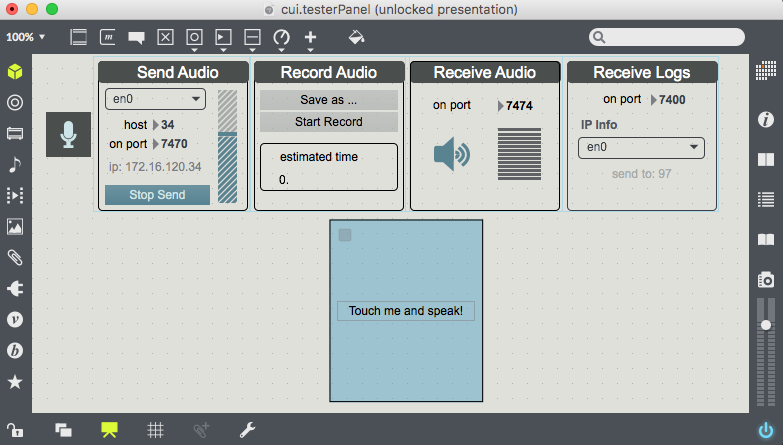
\includegraphics[width=1.0\textwidth]{bilder/3_cptTester.png}    
    \caption{Max Oberfläche mit dem cpt Tester-Panel}
    \label{fig:cpt-tester-panel}
\end{figure}

\textbf{Tester-Panel}\\
Hier sind die verschiedenen Komponenten aus Abbildung \ref{fig:cpt-komponenten} zu sehen. \textit{Send Audio} überträgt die Spracheingaben vom Mikrofon des Rechners an die konfigurierte \textit{\ac{IP}}-Adresse. \textit{Record Audio} zeichnet die Tonspuren auf. Der blau hinterlegte, darunterliegende Bereich bildet die Sprachaktivierung ab. Über die \textit{Receive Audio} Komponente empfängt man die Antwortphrasen des Simulator-Panels. Über die \textit{Logging Komponente} können zusätzliche Textinformationen zum Test gespeichert werden. Das Simulator-Panel, zu sehen in Abbildung \ref{fig:cpt-simulator-panel}, beinhaltet die Gegenstücke zu den eben genannten Komponenten. 

\begin{figure}[!htb]
    \centering
    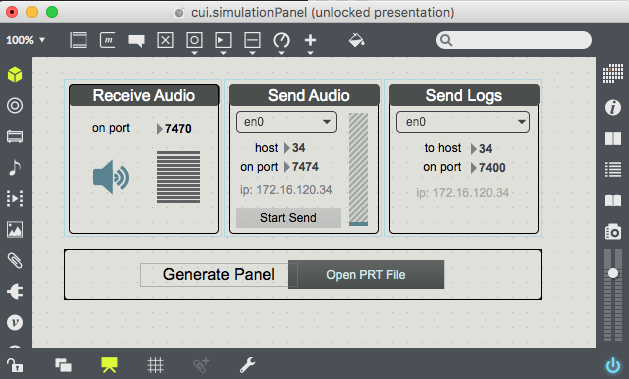
\includegraphics[width=1.0\textwidth]{bilder/3_cptSimulator.png}
    \caption{Max Oberfläche mit dem cpt Simulator-Panel}
    \label{fig:cpt-simulator-panel}
\end{figure}

\textbf{Simulator-Panel}
\textit{Receive Audio} empfängt die Spracheingaben des Testers, während die \textit{Send Audio} Komponente die Antwortphrasen zurück sendet. Über die darunter liegende Schaltfläche kann eine \ac{prt} Ausgabe Datei (\vgl Abbildung \ref{fig:prototyping-toolchain}) geladen werden. Die Oberfläche baut sich im Anschluss dynamisch auf. Dieser Vorgang ist mit entsprechenden Abbildungen in Kapitel \ref{subsec:prototyping-tests} näher beschrieben. Vor Verwendung des \ac{cpt}, müssen zunächst die Audio und Skript Dateien entsprechend generiert werden.\\

\textbf{Skript Datei}\\
Das Skript dient als Mittel zur Kommunikation zwischen den Anwendungen der Toolchain. Als Format wird \textit{\ac{JSON}} verwendet. Im \nameref{sec:Anhang} unter Kapitel \ref{sec:cpt-input-schema} ist das Schema des Skriptes zu finden. Es enthält strukturelle Elemente, wie den Namen des Projektes und des verwendeten Szenarios. Zudem beinhaltet es testspezifische Daten, wie die Namen der Testpersonen und den eigentlichen Dialog-Daten mit den Antworttexten. Diese Daten bilden ein Gesamtszenario ab (hier die erarbeiteten Szenarien aus Kapitel \ref{subsec:szenarien}). Dabei unterscheidet sich die vom \ac{cft} generierte Datei kaum von der aus dem \ac{prt} ausgegebenen. 

\textbf{phrase render tool}\\
Das \ac{prt} wurde vom fachlichen Betreuer der Arbeit implementiert. Abbildung \ref{fig:prt-gui} zeigt die Oberfläche der Anwendung. Über die \textit{Start} Schaltfläche kann das vom \ac{cft} ausgegebene Skript geladen werden. Die Anwendung generiert die entsprechenden Audiodateien und komplettiert die Skript Datei. Es fügt diesem die Pfade der Audiodateien hinzu und modifiziert gegebenenfalls die Antworttexte passend zum generierten Audio. Im Anschluss werden auf der Festplatte die Ordnerstruktur entsprechend des Skriptaufbaus erstellt und sämtliche Dateien darunter abgelegt. 

\begin{figure}[!htb]
    \centering
    
\includegraphics[width=0.7\textwidth]{bilder/3_prtGui.png}
    \caption{prt Oberfläche}
    \label{fig:prt-gui}
\end{figure}

Eine unter \textit{macOS} ausführbare Datei ist auf der beiliegenden CD unter \textit{„Quelltexte/prt/“} zu finden.

\textbf{communication flow tool}\\
Aus zeitlichen Gründen und da es für die Durchführung der Tests nicht zwingend notwendig ist, wird das \ac{cft} nicht im Zuge dieser Arbeit umgesetzt. Daher werden die Szenarien aus Kapitel \ref{subsec:szenarien} händisch in die entsprechenden Skript Dateien transkribiert. Das nächste Kapitel beschreibt die Anwendung der Prototyping Toolchain.

\subsection{Anwendung der Prototyping Toolchain}
\label{subsec:prototyping-tests}
Für die Erarbeitung eines Feinkonzeptes wird die Toolchain für den Aufbau der Benutzertests angewandt. Aufgrund es fehlenden \ac{cft} wird für jedes Szenario aus Kapitel \ref{subsec:szenarien} ein Skript per Hand erstellt. Alle Skripten sind auf der CD unter \textit{„Quelltexte/prototyping\_skripten“} zu finden. Da diese bereits Utterances und Antwortsätze enthalten, fungieren sie als das Grundkonzept und werden durch die Tests erweitert \bzw angepasst.  

\textbf{Testaufbau}\\
Vor jedem Durchlauf wird die Testperson gemäß Lebensumstand einem der Szenarien aus Kapitel \ref{subsec:szenarien} zugeordnet und ihr Name in das Skript eingetragen. Als Beispiel wird das „Partnerschafts“ Szenario aus Abbildung \ref{fig:szenario-partner-anhang} herangezogen. Aus Platz- und Übersichtsgründen ist hier eine vollständige Abbildung nicht möglich. Um den Prozess zu veranschaulichen, dient ein Skriptauszug aus der ersten Aufgabe dieses Szenarios:

\begin{center}
\textit{Prüfe den Eingang deiner Einkünfte.}
\end{center}

Aus dem Schema unter Kapitel \ref{sec:cpt-input-schema} ist bekannt, dass sich das Skript aus Teilszenarien zusammensetzt. Diese beinhalten wiederum Intents. Jeder Intent hat eine oder mehrere Antworten. Listing \ref{lst:skriptauszug-gehalt} zeigt den Skriptauszug für die Beispielaufgabe. 

\begin{lstlisting}[language={HTML},caption={Auszug aus dem Skript des Partnerschaft Szenarios},label={lst:skriptauszug-gehalt}]
{
    "name": "salaryIntent",
    "utterances": ["Gehalt/Lohn da?"],
    "priority": { "main": 0 },
    "responses": [{
            "subject": "SalaryArrived",
            "phrase": "Dein Gehalt fuer diesen Monat ist bereits eingegangen"
        }
    ]
}
\end{lstlisting}

Startet man nun das \ac{prt} und lädt die Skript Datei über die entsprechende Schaltfläche (\vgl Abbildung \ref{fig:prt-gui}), generiert es die Dateien und Ordner gemäß der Schema Struktur, zu sehen in Abbildung \ref{fig:prt-files}.

\begin{figure}[!htb]
    \centering
    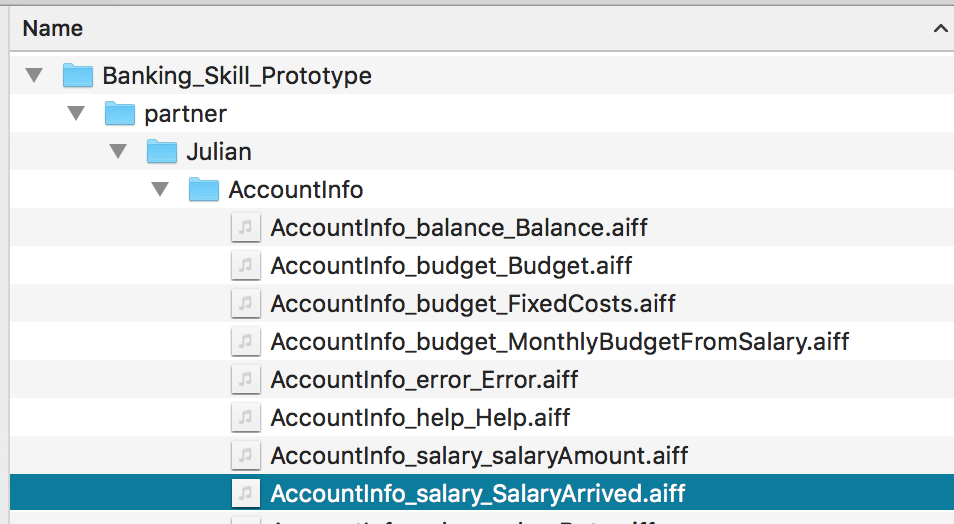
\includegraphics[width=1.0\textwidth]{bilder/3_prtAudio.png}
    \caption{Generierte Ordnerstruktur und Dateien für Partnerschafts Szenario}
    \label{fig:prt-files}
\end{figure}

Der „AccountInfo“ Ordner aus Abbildung \ref{fig:prt-files} enthält alle Audio Dateien für das erste Teilszenario. Die Datei aus dem Beispiel ist blau markiert. \newpage

\begin{lstlisting}[language={HTML},caption={Beispiel-Abschnitt nach der Modifikation durch das prt},label={lst:skriptauszug-gehalt-modifiziert}]
{
          "name" : "salaryIntent",
          "utterances": ["Gehalt/Lohn da?"],
          "priority" : {"main": 0},
          "responses" : [{
              "subject": "SalaryArrived",
              "audio": "AccountInfo_salary_SalaryArrived.aiff",
              "phrase": "Dein Gehalt fuer diesen Monat  ist bereits eingegangen"
            }
          ]
        }
\end{lstlisting} 

Auf gleicher Ebene wie der „AccountInfo“ Ordner, befindet sich das vom \ac{prt} modifizierte Skript. Listing \ref{lst:skriptauszug-gehalt-modifiziert} stellt den geänderten Abschnitt des „salaryIntent“ dar.\\ 
Der Antwortphrase wird vom \ac{prt} das Feld „audio“ hinzugefügt, welches den Namen der entsprechenden Datei enthält (\vgl Abbildung \ref{fig:prt-files}). Nun kann das \ac{cpt} gestartet und die modifzierte Skript Datei geladen werden (\vgl Abbildung \ref{fig:cpt-simulator-panel}), um die Oberfläche für den Test aufzubauen. Für jedes Teilszenario wird ein Reiter erstellt. Diese beinhalten im Idealfall alle Intents die der Tester für die Erfüllung der Aufgabe braucht oder eventuell benutzt. Abbildung \ref{fig:cpt-gui} zeigt den Auschnitt des „AccountInfo“ Reiters der für das Testen der ersten Aufgabe des Partnerschafts Szenarios verwendet wird. Darin zu sehen sind der salaryIntent und dessen Antwortphrase aus dem Beispiel. Durch Klicken auf die Antwort wird diese abgespielt und an das Tester-Panel übertragen. Rechts neben dem hier gezeigten Reiter ist ein weiterer, der alle Intents der zweiten Aufgabe enthält und so weiter.

\begin{figure}[!htb]
    \centering
    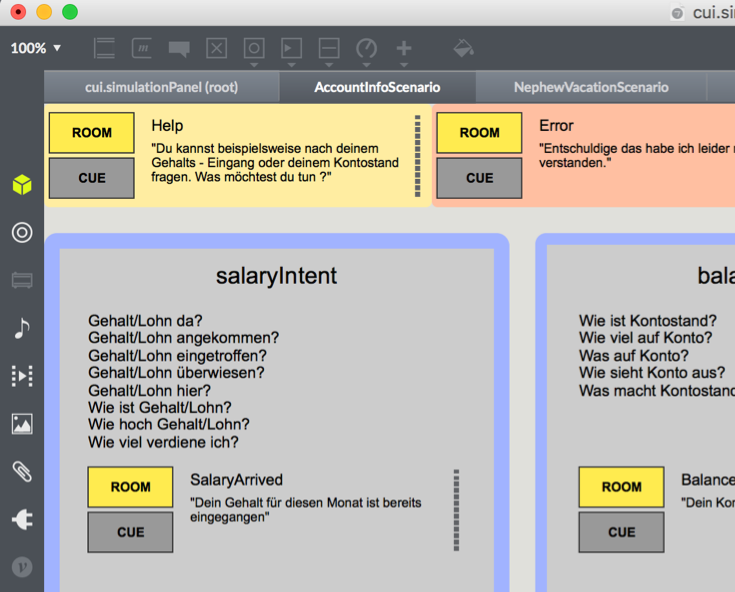
\includegraphics[width=1.0\textwidth]{bilder/3_cptGui.png}
    \caption{cpt GUI für das Testen der ersten Aufgabe im Partnerschaft Szenario}
    \label{fig:cpt-gui}
\end{figure}

Im Testlabor muss das Tester-Panel geöffnet werden. Im Idealfall weiß die Testperson nichts vom Simulator-Panel oder der Person die es steuert. Beide Panele werden mit der \ac{IP}-Adresse des jeweils anderen Rechners und dem entsprechenden Port konfiguriert. Der Aufbau ist damit abgeschlossen und der eigentliche Test kann durchgeführt werden.\\

\textbf{Test Durchführung}\\
Der Testoperator unterweist die Testperson und stellt das Szenario vor. Im Anschluss führt der Tester die vom Operator genannten Aufgaben aus. Abbildung \ref{fig:test-user-woz} zeigt eine der Testpersonen und den im Nebenraum sitzenden \ac{WOz} bei der Durchführung eines Tests.

\begin{figure}[!htb]
  \centering
  \begin{minipage}[b]{0.48\textwidth}
    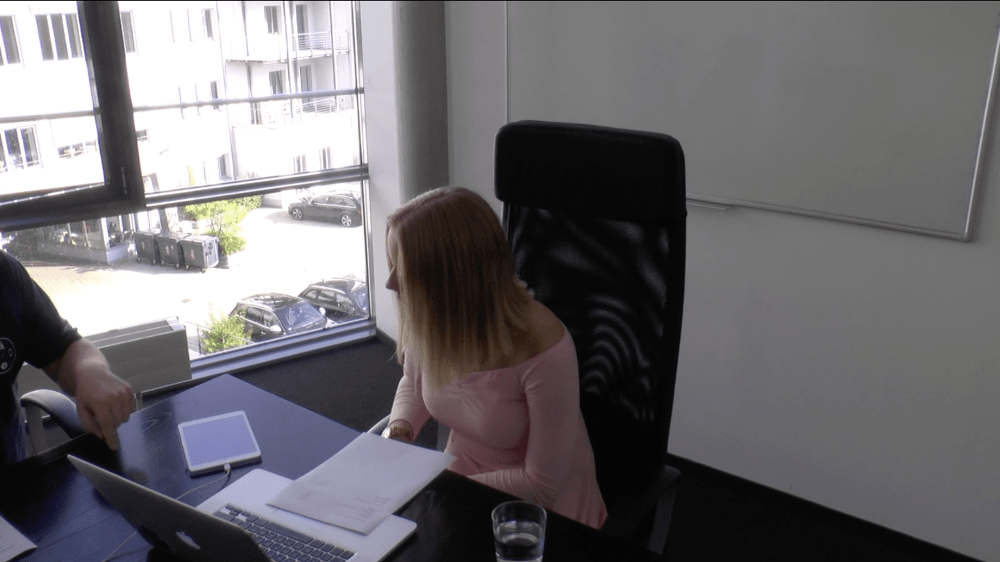
\includegraphics[width=\textwidth]{bilder/3_testUser.png}
  \end{minipage}
  \begin{minipage}[b]{0.48\textwidth}
    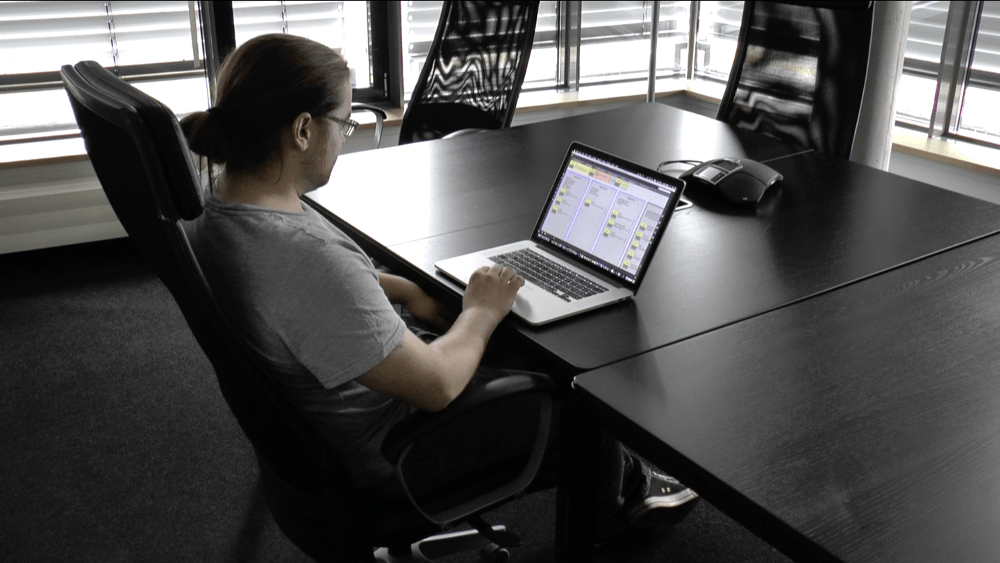
\includegraphics[width=\textwidth]{bilder/3_testWoz.png}
  \end{minipage}
  \caption{Testperson und WOz bei der Durchführung eines Tests}
  \label{fig:test-user-woz}
\end{figure}

Währenddessen notieren der Operator und \ggf der \ac{WOz} Auffälligkeiten und Anmerkungen zum Ablauf. Nach Abschluss der Aufgaben kann der Tester befragt oder das System diskutiert werden. Die Auswertung der Aufnahmen und Notizen erfolgt im Anschluss. Gewonnene Erkenntnisse fließen in die nächste Iteration ein.

\textbf{Test Ergebnisse}\\
Zwölf verschiedene Personen haben die Tests durchgeführt. Obwohl viel Zeit in die Anforderungsanalyse aus Kapitel \ref{sec:requirements-engineering} geflossen ist, hat jeder Test wichtige und sinnvolle Erkenntnisse erschlossen. Darunter auch neue Funktionalitäten, die den User Stories unter Kapitel \ref{sec:anhang-user-stories} hinzugefügt werden.. Im Folgenden wird eine Zusammenfassung gegeben.

\begin{itemize}
 \item Budget der letzten Finanzperiode: Neben der Ausgabe des Budgets der aktuellen Finanzperiode, kann auch das der letzten ausgegeben werden. Denkbar ist auch ein Vergleich beider Budgets. Dadurch ist es Nutzern möglich herauszufinden mit welcher Tendenz zu rechnen ist oder ob Anpassungen im Ausgabeverhalten bereits Wirkung zeigen.
 
 \item Ausgaben der letzten Finanzperiode: Tester haben nach den Ausgaben der letzten Finanzperiode gefragt. Dabei sollen nicht nur Fixkosten, sondern alle Ausgaben einkalkuliert werden.
 
 \item Sparziele ausgeben: Neben der Verwaltung soll es auch möglich sein alle Sparziele auszugeben.
 
 \item Fixkosten: Neben der Höhe der Fixkosten haben Tester auch gefragt, woraus sich die Fixkosten zusammen setzen. Eine Auflistung aller regelmäßigen Ausgaben ist denkbar.
 
 \item Transaktion mit IBAN: In Kapitel \ref{subsec:user-stories} ist konzipiert, dass Transaktion nur über vorher angelegte Vorlagen durchgeführt werden können. Bei Verwendung eines \ac{IBAN}, sollen Benutzer auf eine grafische Anwendung \bzw Überweisungsträger zurückgreifen. Eine der Testpersonen trägt eine Gleitsichtbrille. Sie hat folgendes sinngemäß angegeben: 
 \textit{Möchte man eine \ac{IBAN} von einem Blatt Papier, zum Beispiel einer Rechnung, ablesen und unter Verwendung einer Online-Banking-Anwendung eingeben, ist das ständige Hin- und Herwechseln zwischen Papier und Bildschirm unangenehm. Es wäre wesentlich einfacher die \ac{IBAN} vom Papier abzulesen und einem Gerät zu diktieren. Dabei muss man nicht einmal die Augen vom Papier abwenden}.
 
 \item Höhe und Überweisungsdatum des Gehaltes prüfen: Neben der Information, ob das Gehalt bereits überwiesen wurde, haben viele der Tester nach der Höhe des Gehaltes gefragt. Auch das Überweisungsdatum scheint von Interesse zu sein.
\end{itemize}

Die hier erlangten Ergebnisse zeigen, wie wichtig der Einsatz von Prototyping ist.\\
Das über die Tests iterativ entwickelte Konzept soll nun in eine einheitliche, schriftliche Form gebracht werden. Da ein Alexa Skill gemäß Kapitel \ref{sec:alexa-voice-service} in Intents organisiert ist, wird das Konzept auch auf diese Weise dokumentiert. Jeder Intent wird nach aktuellem Kenntnisstand identifiziert und über dessen Slots, in den empirischen Daten und Tests gesammelten Utterances und Antwort-Beispielen definiert. Aus Gründen der Übersichtlichkeit und Lesbarkeit, wird nur einer dieser Intents beschrieben.

\begin{figure}[!htb]
    \centering
    \fbox{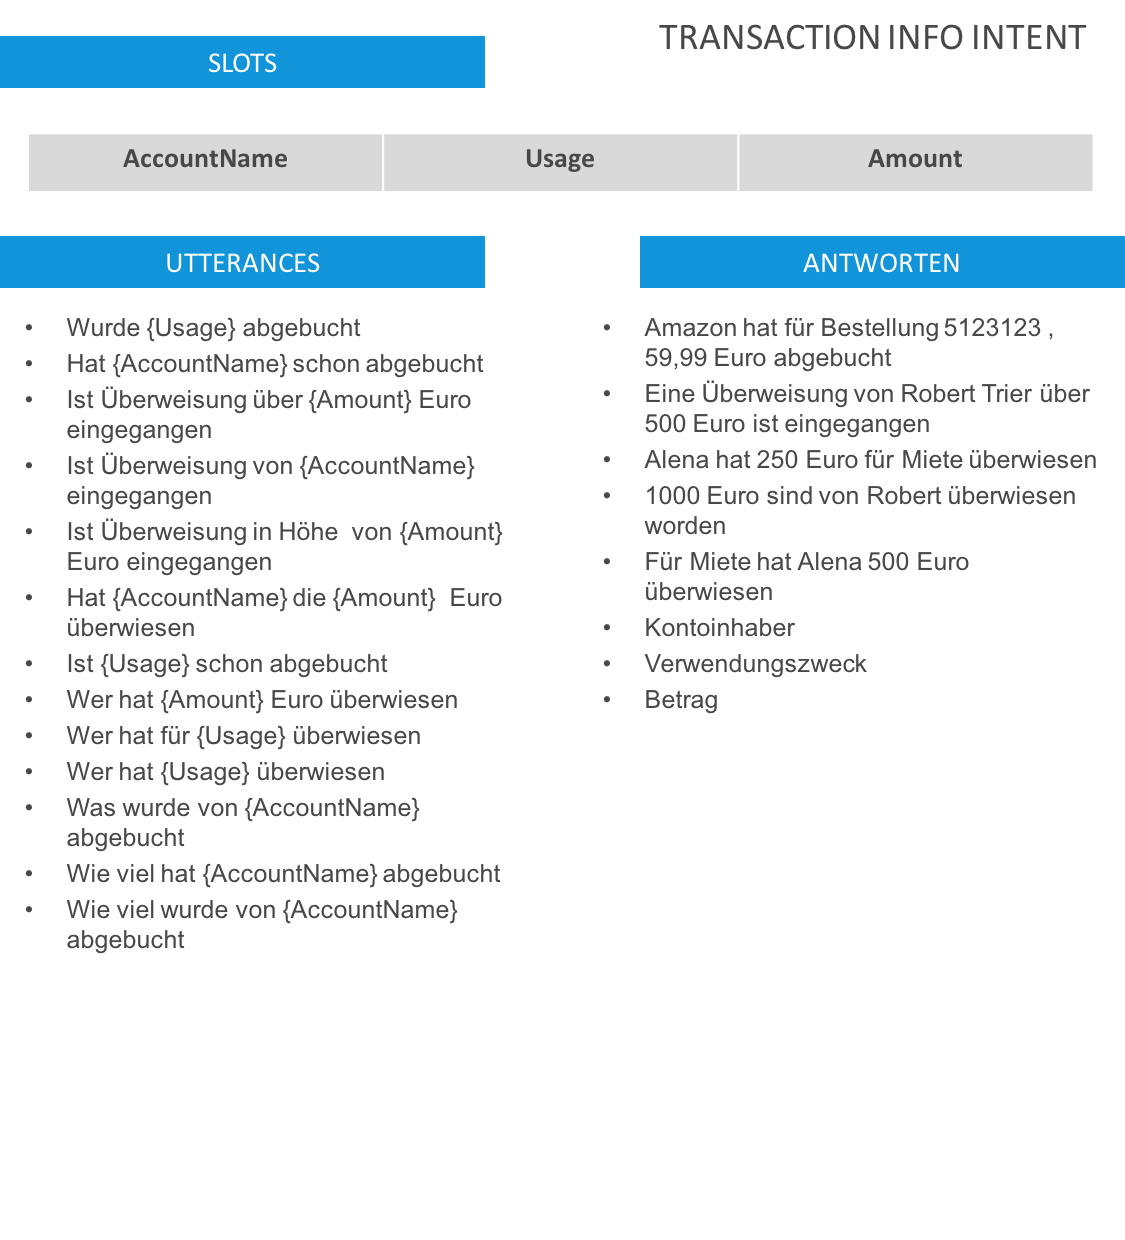
\includegraphics[width=1.0\textwidth]{bilder/3_conceptTransactionInfo.png}}
    \caption{Ausgearbeiteter Transaktions-Info Intent}
    \label{fig:conception-transaction-info}
\end{figure}

Sämtliche Intents sind im Anhang unter Kapitel \ref{sec:anhang-konzept} zu finden. Abgesehen von etwaigen Änderungen die für die Umsetzung notwendig sind, wird das Konzept im weiteren Verlauf der Arbeit nicht weiter ausgebaut. An dieser Stelle sei jedoch erwähnt, dass das Bedienkonzept einer \ac{CUI} Anwendung auch lange nach der Auslieferung intensiv erweitert werden muss. Die hier erarbeiteten Formulierungen bilden lediglich eine kleine Basis dessen ab, was der Skill verstehen sollte. Abbildung \ref{fig:conception-transaction-info} zeigt die Ausarbeitung des „TransactionInfoIntent“. Gemäß Kapitel \ref{sec:ziel-der-arbeit}, werden Teile dieses Konzeptes in Kapitel \ref{cha:umsetzung} umgesetzt.\\

\section{Sicherheits-Konzept}
\label{sec:sicherheits-konzept}
Bei den User Stories 2-5 aus Kapitel \ref{sec:anhang-user-stories} geht es um die Authentifizierung \bzw die Registrierung von Benutzern. Unter Verwendung von Alexa gibt es jedoch ein Problem. Man kann nicht zwischen den Personen differenzieren, die in den Echo sprechen. Alexa Endgeräte sind zwar über einen bestimmten Benutzer mit dessen Amazon Account eingerichtet, dennoch kann das Gerät von mehreren Personen verwendet werden. Der Echo \bzw Echo Dot wird überwiegend zu Hause benutzt. Theoretisch hat jeder im Haus Zugang zum Lautsprecher, egal ob Familie, eingeladene Freunde, die Haushaltshilfe oder ein Einbrecher. Dabei wäre es fatal, wenn ein Banking Skill nicht zwischen diesen Personen unterscheiden kann und jedem Zugang zum Bankkonto des Echo-Besitzers gewährt. Genauso ist irgendeine Art von Passwort, die man in das Gerät spricht wenig zielführend. Der Weg bis zum Mikrofon ist unverschlüsselt und jede Person in unmittelbarer Nähe kann mithören. Amazon arbeitet im Moment an einer Stimmenerkennung \cite{alexa-voice-recognition}, jedoch ist noch nicht bekannt wann diese in Deutschland verfügbar ist.\\
In der Umfrage aus Kapitel \ref{subsec:online-umfrage} gibt einer der Befragten an, dass es effizienter wäre sich über das Smartphone mit Fingerabdruck statt einem Passwort zu authentifizieren. Zwar ist damit eine Online-Banking-Anwendung gemeint, jedoch kann man den Gedanken trotzdem aufgreifen. Statt über den Echo wäre es auch möglich, Benutzer des Banking-Skills über ihr Smartphone zu authentifizieren. Abbildung \ref{fig:security-concept} zeigt ein denkbares Konzept.

\begin{figure}[!htb]
    \centering
    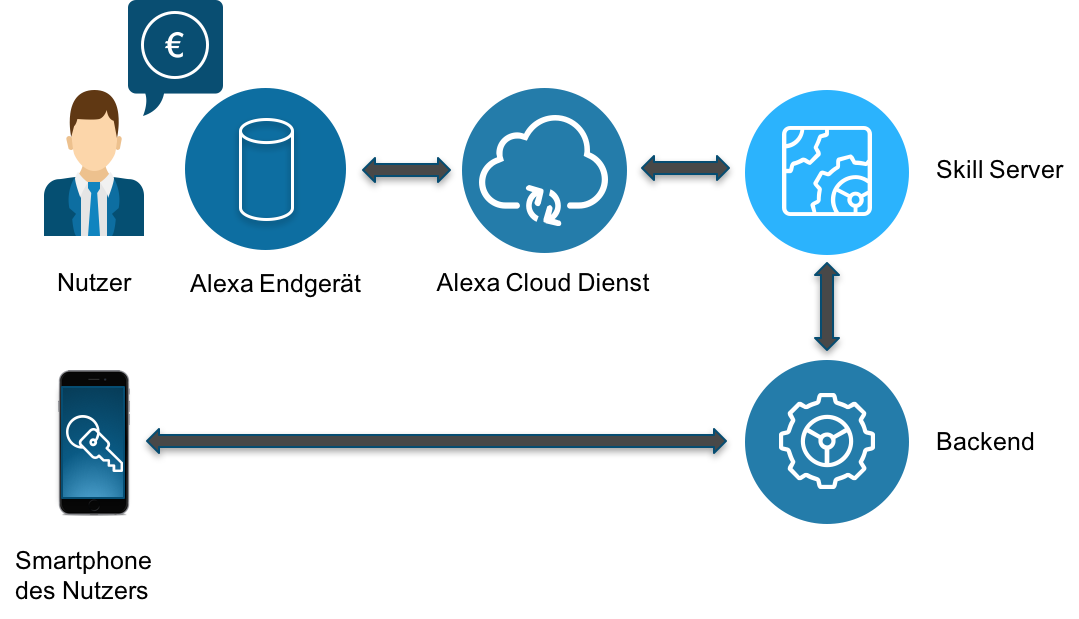
\includegraphics[width=1.0\textwidth]{bilder/3_securityConcept.png}
    \caption{Konzept für Authentifizierung}
    \label{fig:security-concept}
\end{figure}

Das Backend für die Registrierung ist bewusst als eigenständige Instanz und nicht als Teil des Skill-Servers konzipiert. Da dieser Mechanismus auch für andere \acp{VUI} Systeme (Cortana, Siri, \etc) funktionieren kann, ist man so unabhängig von der verwendeten Plattform.\\
Bevor ein Benutzer den Banking Skill verwenden kann, muss er sich zunächst über eine Smartphone App beim entsprechenden Server registrieren. Beim Starten oder bei Verwendung des Banking Skills, kann das System den Nutzer beispielsweise nach seinem Namen fragen. Im Anschluss wird geprüft, ob der Name bereits registriert ist. Daraufhin wird die Aufforderung zur Authentifizierung via \textit{Push Notification} an das Smartphone des Benutzers gesendet. Um den Gedanken aus der Umfrage aufzugreifen, ist hier eine Bestätigung per Fingerabdruck denkbar. Da der schnellere Zugang einer der Gründe für die Nutzung des Skills ist, stellt eine Fingerabdruck Abfrage einen guten Kompromiss zwischen Sicherheit und Effizienz dar. Erst wenn der Sprechende authentifiziert ist kann er alle Funktionen des Skill nutzen.\\
Alle Teilnehmer der Umfrage, der Interviews und User Tests haben große Sicherheitsbedenken. Auch wenn ein solcher Mechanismus Zeit kostet, wirkt sich dessen Verwendung möglicherweise positiv auf sicherheitskritische Nutzer aus. Es gibt noch einen Vorteil den dieses Konzept mit sich bringt. Die schützenswerten Daten für die Authentifzierung passieren dabei nicht die Amazon Plattform. Der Austausch findet abseits zwischen Smartphone-Anwendung und Backend statt. Die Informationen die an Alexa übertragen werden sind lediglich der Name des Benutzers und die Bestätigung, dass dieser authentifiziert ist.\\
Auch wenn die Stimmenerkennung für Alexa veröffentlicht wird, ist das hier beschriebene Konzept sinnvoll und kann als zusätzliche Maßnahme für mehr Sicherheit sorgen. Als Teil der Umsetzung in Kapitel \ref{cha:umsetzung} sind dort weitere Details dazu beschrieben.